\chapter{Empirical Evaluation}\label{ch:empirical-evaluation}

\section{Dataset Analysis}\label{sec:empirical-evaluation:dataset-analysis}
This section presents an analysis of the three datasets used in our empirical evaluation: \textit{FactBench}, \textit{YAGO}, and \textit{DBpedia}.
Each dataset offers unique characteristics and challenges, providing a comprehensive basis for assessing our knowledge graph fact verification system.
\subsection{FactBench Dataset}\label{subsec:empirical-evaluation:dataset-analysis:factbench}
\textit{FactBench} is a multilingual dataset specifically designed for fact-checking in knowledge graphs~\footnote{\url{https://github.com/DeFacto/FactBench}}~\cite{GERBER201585}.
It comprises 2,800 facts, 1.500 true and 1.300 false, across three languages: English, German, and French.
The dataset covers various domains, including geography, politics, and entertainment.
The data was automatically extracted from Wikipedia\footnote{\url{https://www.wikipedia.org/}} (DBpedia respectively) and Freebase\footnote{\url{https://developers.google.com/freebase}}.

To obtain positive examples, the authors leverages facts from both DBpedia and Freebase.
For each property under consideration, they generated these examples by issuing either a SPARQL (for DBpedia) or MQL (for Freebase) query.
They then selected the top 150 results.
In Freebase, results are ranked using an internal relevance score, while in \textit{DBpedia}, the results are sorted by the number of inbound links to the resource’s corresponding Wikipedia page.
In total, 1500 correct statements were collected, with 750 allocated to both the test and training sets, ensuring that each relation had 150 positive facts equally distributed between the test and training sets.

For generating incorrect facts (negative examples), the authors modified correct ones while adhering to domain and range constraints.
To ensure that the negative examples closely resemble true statements (\ie, meaningful triples), the team altered the positive examples while still adhering to domain and range restrictions.
Given a triple (s, p, o) and its timespan (from, to) from the knowledge base, they used different methods to generate sets of negative examples.
These methods include modifying the subject, object, both subject and object, or the property.
Additionally, they included random modifications, a 20\% mix of these methods, and variations in the date.

We don't consider the time aspect in our evaluation, as our system is not designed to handle time-sensitive issues.
We consider a configuration where incorrect facts are a mix produced using different negative example generation strategies, resulting in a ground-truth accuracy of $\mu$ = 0.54.
Key characteristics of \textit{FactBench} include:
\begin{itemize}
    \item Multilingual support (English, German, and French)
    \item Diverse fact types, including domain-specific and temporal facts
    \item Manually curated for high-quality ground truth
\end{itemize}

In our analysis, we found that \textit{FactBench} presents a balanced challenge for our system, with a mix of straightforward and complex fact verification tasks.
\subsection{YAGO Dataset}\label{subsec:empirical-evaluation:dataset-analysis:yago}
YAGO (Yet Another Great Ontology) is a large-scale knowledge base derived from Wikipedia, WordNet~\footnote{\url{https://wordnet.princeton.edu/}}, and GeoNames~\footnote{\url{https://www.geonames.org/}}.
For our evaluation, we use \textit{YAGO2-sample}~\footnote{\url{https://aclanthology.org/attachments/D17-1183.Attachment.zip}}~\cite{ojha-talukdar-2017-kgeval}, a subset of the full YAGO2 knowledge graph derived from AMIE horn clauses~\cite{Yago_AMIE}.
This sample consists of 1,386 beliefs spanning 16 unique predicates.

Key characteristics of the \textit{YAGO} dataset in our evaluation include:
\begin{itemize}
    \item High accuracy: The gold standard accuracy of the \textit{YAGO2-sample} is 99.20\%, indicating a very high-quality dataset.
    \item Diverse predicates: The sample covers 16 different predicates, allowing for evaluation across a range of relationship types.
    \item Balanced distribution: Unlike domain-specific datasets, \textit{YAGO2-sample} covers a broad range of topics, reflecting the diverse nature of Wikipedia.
\end{itemize}

The high accuracy of the \textit{YAGO2-sample} presents a unique challenge for our evaluation system.
\subsection{DBpedia Dataset}\label{subsec:empirical-evaluation:dataset-analysis:dbpedia}
\textit{DBpedia} serves as a comprehensive, large-scale knowledge base derived from Wikipedia, offering structured information about millions of entities.
For our evaluation, we utilize \textit{DBpedia} version 2015-10 which contains approximately 6.2M entities and 1.1B triplets.
Following Marchesin et al.'s approach~\cite{Marchesin_Silvello_Alonso_2024} to entity-oriented research, several filtering criteria were applied to ensure high-quality data for evaluation.

The analysis was restricted to subject entities that include both: 1) rdfs:label predicate and 2) rdfs:comment predicate

Additionally, they focused exclusively on A-Box triplets (assertional knowledge) while excluding T-Box triplets (terminological knowledge).
The T-Box encompasses ontological entities and relationships, while A-Box contains the actual assertions that need verification.
After applying these filters, their working dataset consisted 4.6M entities with 170M triplets.

From this filtered dataset, they conducted a comprehensive annotation study on 9,930 facts, which were carefully selected to represent diverse types of relationships and knowledge domains within \textit{DBpedia}.
To ensure annotation quality, Marchesin et al. implemented several measures:
\begin{itemize}
    \item Multiple annotators per fact (minimum of three annotations per triplet)
    \item Expert consensus requirement for final labels
    \item Binary validation approach treating all incorrect facts equally regardless of error type
    \item Documented agreement rates between expert annotators (77\% agreement with Cohen's κ score of 0.51)
    \item Third-party resolution for 82\% of initial disagreements
\end{itemize}

The dataset was carefully curated to ensure a manageable yet representative evaluation set, derived from the vast scale of \textit{DBpedia}.
By utilizing this curated subset of \textit{DBpedia}, we benefit from a balance between the richness of a real-world knowledge graph and the practicality required for thorough empirical evaluation.
For our evaluation system, we use subset of this annotated dataset, by removing facts with \textit{<UNK>} labels, resulting in 9,344 facts.

\paragraph{Dataset Summary:}\label{par:summary}
To conclude, our empirical evaluation utilizes three distinct datasets: \textit{FactBench}, \textit{YAGO}, and \textit{DBpedia}.
Each dataset offers unique characteristics that allow us to assess our knowledge graph veracity framework across diverse scenarios.
Table~\ref{tab:dataset-summary} summarizes the key features of these datasets:

\begin{table}[h!]
    \centering
    \caption{Statistical summary of FactBench, YAGO, and DBpedia datasets}
    \begin{tabular}{lccc}
        \toprule
        & \textbf{FactBench} & \textbf{YAGO} & \textbf{DBpedia} \\
        \midrule
        Num. of Facts & 2,800 & 1,386 & 9,344 \\
        Num. of Predicates & 10 & 16 & 1,092 \\
%        Query-Entity Pairs & N/A & N/A & N/A \\
        Avg. Facts per Entity & 2.42 & 1.69 & 3.18 \\
        Gold Accuracy ($\mu$) & 0.54 & 0.99 & 0.85 \\
        \bottomrule
    \end{tabular}
    \label{tab:dataset-summary}
\end{table}

\textit{FactBench} provides a good distribution of true and false statements across multiple domains, offering a robust testbed for fact verification.
\textit{YAGO}, with its high accuracy, challenges our framework to detect subtle inaccuracies in an otherwise highly reliable knowledge graph.
The \textit{DBpedia} subset, curated specifically for entity-oriented search tasks, allows us to evaluate our framework in the context of query-dependent fact checking.
This diverse selection of datasets enables a comprehensive evaluation of our veracity estimation framework.

\section{Candidate Models}\label{sec:empirical-evaluation:candidate-models}
\subsection{Gemma2}\label{subsec:empirical-evaluation:candidate-models:gemma2}
Gemma is a family of lightweight, state-of-the-art open models from Google, built from the same research and technology used to create the Gemini models~\footnote{\url{https://deepmind.google/technologies/gemini/#introduction}}.
They are text-to-text, decoder-only large language models, available in English, with open weights for both pre-trained variants and instruction-tuned variants.
Gemma 2 implements a similar architecture to the original Gemma model, with a few key differences.
The model alternates between local sliding window attention with a 4096-token span and global attention with an 8192-token span in alternate layers.
Logits are capped within a specified range to stabilize the values during attention and final layers, with soft\_cap set to 50 for self-attention layers and 30 for the final layer.
RMSNorm is used for normalization in transformer sub-layers, and \ac{GQA} with two groups enhances inference speed without sacrificing performance.
This hybrid approach aims to balance efficiency with the ability to capture long-range dependencies in the input.

We selected the \textit{Gemma2-9B} model for our evaluation, which has 9 billion parameters.
The 9B model learns from a larger teacher model during initial training in pre-training and use on-policy distillation to refine its performance post-training.
This approach allows \textit{Gemma2-9B} to capture the knowledge and capabilities of the larger model while maintaining a more compact size.
As a result, \textit{Gemma2-9B} delivers competitive performance relative to models 2-3 times its size, making it an attractive choice for applications with computational constraints.

\subsection{Qwen2.5}\label{subsec:empirical-evaluation:candidate-models:qwen2.5}
\textit{Qwen2.5} is the latest series of Qwen LLMs~\cite{qwen2}.
For \textit{Qwen2.5}, Alibaba Cloud~\footnote{\url{https://www.alibabacloud.com/en?_p_lc=7}} release a number of base language models and instruction-tuned language models ranging from 0.5 to 72 billion parameters.
All models are pre-trained on our latest large-scale dataset, encompassing up to 18 trillion tokens.
Compared to \textit{Qwen2}, \textit{Qwen2.5} has acquired significantly more knowledge and has greatly improved capabilities in coding and mathematics.
Additionally, the new models achieve significant improvements in instruction following, generating long texts (over 8K tokens), understanding structured data (\eg, tables), and generating structured outputs especially JSON.
\textit{Qwen2.5} models are generally more resilient to the diversity of system prompts, enhancing role-play implementation and condition-setting for chatbots.
Like \textit{Qwen2}, the \textit{Qwen2.5} language models support up to 128K tokens and can generate up to 8K tokens.
They also maintain multilingual support for over 29 languages~\cite{qwen2.5}.

We selected the \textit{Qwen2.5-7b} model for our evaluation, which has 7 billion parameters.

\subsection{Llama3.1}\label{subsec:empirical-evaluation:candidate-models:llama3.1}
The Meta \textit{Llama3.1} collection of multilingual LLMs is a collection of pre-trained and instruction tuned generative models in 8B, 70B and 405B sizes (text in/text out).
The \textit{Llama3.1} instruction tuned text only models (8B, 70B, 405B) are optimized for multilingual dialogue use cases and outperform many of the available open source and closed chat models on common industry benchmarks.

\textit{Llama3.1} is an auto-regressive language model that uses an optimized transformer architecture.
\textit{Llama3.1} was pre-trained on ~15 trillion tokens of data.
In post-training The models produced by doing several rounds of alignment on top of the pre-trained model.
Each round involves \ac{SFT}, \ac{RS}, and \ac{DPO}.
Meta use synthetic data generation to produce the vast majority of our SFT examples, iterating multiple times to produce higher and higher quality synthetic data across all capabilities.
Additionally, they invest in multiple data processing techniques to filter this synthetic data to the highest quality.
This enables model to scale the amount of fine-tuning data across capabilities.
Compared to previous versions of Llama, developers improved both the quantity and quality of the data we use for pre and post-training.
These improvements include the development of more careful pre-processing and curation pipelines for pre-training data, the development of more rigorous quality assurance, and filtering approaches for post-training data~\cite{dubey2024llama3herdmodels,meta2023llama3}.

We selected the \textit{Llama3.1-8b} model for our evaluation, which has 8 billion parameters.

\subsection{Mistral}\label{subsec:empirical-evaluation:candidate-models:mistral}
The \textit{Mistral} model, released by Mistral AI~\footnote{\url{https://mistral.ai/}}, is a high-performance LLM, designed to outperform larger models in efficiency and effectiveness.
With innovations such as \ac{GQA} and \ac{SWA}, Mistral offers faster inference and better handling of long sequences, reducing computation costs while maintaining high performance~\cite{jiang2023mistral7b,mistral7b_2023}.

We selected the \textit{Mistral-7b} model for our evaluation, which has 7.3 billion parameters, its structure allows it to be both cost-effective and memory efficient, making it suitable for a wide variety of real-world applications

\paragraph{Candidate Model Summary:}\label{par:summary2}
The selection of candidate models for our system was guided by the need for diversity, efficiency, and reliability in processing fact verification tasks within knowledge graphs.
We chose \textit{Gemma2}, \textit{Qwen2.5}, \textit{Llama3.1}, and \textit{Mistral} for their specific strengths in handling diverse linguistic queries, reasoning capabilities, and compatibility with RAG pipelines.
Each of these models brings unique advantages to our verification framework, as summarized in Table~\ref{tab:candidate_models}.

\begin{table}[h!]
    \footnotesize
    \caption{Summary of key strengths of selected candidate LLMs for knowledge graph fact verification.}
    \begin{xltabular}{\linewidth}{cp{3.6cm}X}
        \toprule
        \textbf{Model} & \textbf{Key Strengths} & \textbf{Description} \\
        \midrule
        \multirow{3}{*}{Gemma2} & \multirow{3}{*}{\shortstack{Dense Retrieval \\\& Query Processing}} & Optimized for dense retrieval tasks, Gemma2 processes complex linguistic structures, making it well-suited for entity-rich query generation and document ranking. \\
        \hline
        \multirow{4}{*}{Qwen2.5} & \multirow{4}{*}{\shortstack{Logical Reasoning \\\& Prompt Efficiency}} & Excels in reasoning tasks with minimal prompting. Its accuracy in logical inference supports consistent veracity assessments, especially for ambiguous or conflicting evidence. \\
        \hline
        \multirow{5}{*}{Llama3.1} & \multirow{5}{*}{Efficiency \& Versatility} & Offers a balance of efficiency and accuracy, with robust performance across fact-checking benchmarks. Llama3.1's lower computational demands ensure responsive processing without compromising output quality. \\
        \hline
        \multirow{4}{*}{Mistral} & \multirow{4}{*}{\shortstack{Context Sensitivity \\\& Interpretability}} & Known for nuanced, context-driven outputs and interpretability. Mistral’s language generation capabilities provide clear, human-like explanations, making it ideal for understanding the facts like a human. \\
        \bottomrule
    \end{xltabular}
    \label{tab:candidate_models}
\end{table}

For model selection, we can choose either instruction-tuned and quantized models with similar architectures or with different architectures.
Here, we opted for models with varied architectures to make the ensemble more versatile and capable of handling a wide range of query scenarios.
Using diverse models in the ensemble offers a balanced approach to complex fact verification tasks across knowledge graphs.
This multi-model setup enhances adaptability and reliability, allowing the system to respond accurately to diverse verification scenarios, even when they differ in nature.

\section{Experimental Setup}\label{sec:empirical-evaluation:experimental-setup}
\subsection{Performance Metrics and Evaluation}\label{subsec:empirical-evaluation:experimental-setup:performance-metrics-and-evaluation}
Performance metrics are essential in assessing the efficacy, efficiency, and reliability of a system or model.
The selection of metrics mostly depends on the characteristics of the task, the data, and the objectives.
This section emphasizes the principal performance metrics typically employed in systems utilizing LLMs, information retrieval, and various machine learning tasks.
\paragraph{Correct and Incorrect Criteria:}
The system incorporates explicit CORRECT and INCORRECT states, indicating a binary evaluation mechanism for overall performance.
This fundamental assessment provides a clear, high-level indication of the system's success in handling queries.
\paragraph{Relevance and Accuracy Metrics:}
The evaluation of a fact-checking system typically involves assessing both the correctness and relevance of responses.

Potential metrics include:
\begin{itemize}
    \item \textbf{F1 Score:} The harmonic mean of precision and recall, providing a balanced measure of accuracy.
    \item \textbf{Accuracy:} The proportion of correct responses generated by the system.
\end{itemize}
\paragraph{Latency and Efficiency Measures:}
Given the complexity of the pipeline, evaluating its operational efficiency is crucial:
\begin{itemize}
    \item \textbf{Response Time:} Measuring the end-to-end time from query input to response generation.
    \item \textbf{Component-wise Latency:} Assessing the processing time of individual pipeline components (\eg, embedding generation, LLM processing). Fully reported in ablation study in chapter~\ref{ch:ablation} and performance report in section~\ref{sec:performance-report}.
    \item \textbf{Cost Efficiency:} Evaluating the cost-effectiveness of the pipeline in terms of computational resources and infrastructure by reporting the average token used per query.
\end{itemize}

\paragraph{Consistency Evaluation:}
The use of multiple models and a conflict resolution mechanism necessitates specific evaluation of output consistency:

\begin{itemize}
    \item \textbf{Stability Across Models:} Assessing the consistency of responses generated by different LLMs for the same query, refer to Algorithm~\ref{alg:stability-across-queries}.
\end{itemize}
\begin{algorithm}
    \footnotesize
    \caption{Calculate Model Consistency Per Model}
    \begin{algorithmic}[1]
        \Procedure{ModelStabilityCal}{$models$} \Comment{Containing binary results}
            \State $m\_len \gets \text{length}(models)$, $stabilityScores \gets []$

            \For{$i \gets 0$ to $m\_len - 1$}
                \State $m1 \gets models[i]$, $mStabilities \gets []$

                \For{$j \gets 0$ to $m\_len - 1$}
                    \If{$i \neq j$}
                        \State $m2 \gets models[j]$, $matchCount \gets 0$
                        \State $totPreds \gets \text{length}(m1)$

                        \For{$k \gets 0$ to $totalPredictions - 1$}
                            \If{$m1[k] = m2[k]$}
                                \State $matchCount \gets matchCount + 1$
                            \EndIf
                        \EndFor

                        \State $mStabilities$ \gets $\dfrac{matchCount}{totPreds}$ \Comment{Append the stability score}
                    \EndIf
                \EndFor

                \State $stabilityScores[i] \gets \text{mean}(mStabilities)$
            \EndFor

            \State \Return $stabilityScores$ \Comment{Dictionary with model stability scores}
        \EndProcedure
    \end{algorithmic}
    \label{alg:stability-across-queries}
\end{algorithm}

\subsection{System Configurations}\label{subsec:empirical-evaluation:experimental-setup:system-configurations}
The system configurations are selected based on the best results obtained from black-box testing the pipeline through a series of experiments, detailed in chapter~\ref{ch:ablation}.
Table~\ref{tab:system-configurations} summarizes the key system configurations used in our empirical evaluation.

{
    \noindent
    \centering
    \footnotesize
    \begin{tabularx}{\linewidth}{lp{2.9cm}X}
        \caption{System configurations for empirical evaluation} \\
        \toprule
        \textbf{Section} & \textbf{Parameter} & \textbf{Considerations} \\
        \midrule
        \multirow{4}{*}{Human Understanble Text} & \multirow{4}{*}{Gemma2:9b} & Other LLMs can be used, but using instruction-tuned models is recommended. This is skipped for \textit{FactBench} dataset as discussed on~\ref{subsec:human-understandable-text-generation}. \\
        \hline
        \multirow{3}{*}{Question Generation} & \multirow{3}{*}{Gemma2:9b} & Other LLMs can be used, but using instruction-tuned models is recommended. \\
        \hline
        \multirow{2}{*}{Question Relevance} & Jina-reranker-v1-turbo-en & Cross-encoder models are recommended for this task. \\
        \hline
        Question RelevanceThreshold  & 0.5 & -- \\
        \hline
        Num. of Selected Questions & 3 & -- \\
        \hline
        \multirow{6}{*}{Google Search} & \multirow{6}{*}{--} & Used query params: \textit{lr} = 'lang\_en', \textit{gl} = 'us', \textit{hl} = 'en', \textit{num} = '100'. The lr parameter is set to the language of the query, gl to the country, hl to the language, and num to the number of results. \\
        \hline
        Num. of Selected Documents & 10 & -- \\
        \hline
        \multirow{8}{*}{Document Selection} & \multirow{8}{*}{\shortstack{ms-marco-MiniLM\\-L-6-v2}} & Filtered out the documents from these origins: dbpedia, wikipedia, wikimedia, wikidata, quora, britannica, scholarpedia, newworldencyclopedia, everipedia, encyclopedia, wikibooks, wiktionary, wikiversity, wikisource, wikiquote, wikivoyage, academia, and nytimes \\
        \hline
        Embedding Model & bge-small-en-v1.5 & -- \\
        \hline
        \multirow{2}{*}{Chunking Strategy} & Sliding Window window size 3 & -- \\
        \hline
        Similarity Cut-off & Simple & Use the threshold to filter out irrelevant documents. \\
        \hline
        Similarity Cut-off Threshold & 0.3 & -- \\
        \hline
        Top\_k & 6 & -- \\
        \hline
        \multirow{4}{*}{Tie-Breaking} & \multirow{4}{*}{--} & Use model with higher-param for each model, for llama3.1:8b~$\rightarrow$~70b, gemma2:9b~$\rightarrow$~27b, qwen2.5:7b~$\rightarrow$~14b, and mistral:7b~$\rightarrow$~mistral nemo:12b. \\
        \bottomrule
        \label{tab:system-configurations}
    \end{tabularx}
}

The tests are run on a server with the following specifications:
\begin{itemize}
    \item \textbf{Model Name:} Mac Studio
    \item \textbf{Model Identifier:} Mac14,14
    \item \textbf{Model Number:} Z180000M3T/A
    \item \textbf{Chip:} Apple M2 Ultra
    \item \textbf{Total Number of Cores:} 24 (16 performance and 8 efficiency)
    \item \textbf{Memory:} 192 GB
    \item \textbf{System Firmware Version:} 11881.1.1
    \item \textbf{OS Loader Version:} 11881.1.1
\end{itemize}

\section{Comparative Analysis}\label{sec:empirical-evaluation:comparative-analysis}
\begin{table}[ht!]
    \noindent
    \caption{Empirical evaluation results of the proposed system and candidate LLMs over the FactBench, YAGO, and DBpedia.}
    {\scriptsize ms-marco-MiniLM-L-6-v2, BAAI/bge-small-en-v1.5, Sliding Window (ws 3), Similarity Cut-off (Original), Top\_k 6}
    \resizebox{\textwidth}{!}{
        \begin{threeparttable}
            \begin{tabular}{llcccc||cc}
                \toprule
                \textbf{Dataset}            & \textbf{Model}                     & \textbf{Consistency}\tnote{*}  & \shortstack{\textbf{Avg.}\\\textbf{request time}}                                & \shortstack{\textbf{Avg.}\\\textbf{input tokens}} & \shortstack{\textbf{Avg.}\\\textbf{output tokens}} & \textbf{Acc} & \textbf{F1} \\
                \midrule
                \multirow{6}{*}{FactBench}  & Gemma2                             & 0.8738                         & 2.32s                            & 1509.30                                       & 19.95            & 0.9014    & 0.9085   \\
                                            & Qwen2.5                            & 0.8747                         & 2.46s                            & 1509.18                                       & 67.73            & 0.8746    & 0.8910   \\
                                            & LLama3.1                           & 0.8296                         & 2.87s                            & 1509.24                                       & 104.65           & 0.8243    & 0.8378   \\
                                            & Mistral                            & 0.8686                         & 1.73s                            & 1509.17                                       & 8.81             & 0.8507    & 0.8729   \\ \cline{2-8}
                                            & Most (Qwen2.5:14b)                 & --                             & 27.66s                           & 1509.18                                       & 57.44            & 0.9057    & 0.9145   \\
                                            & Least (Llama3.1:70b)               & --                             & 12.70s                           & 1749.14                                       & 8.73             & 0.9025    & 0.9124   \\ \hline \hline
                \multirow{6}{*}{YAGO}       & Gemma2                             & 0.8882                         & 2.15s                            & 1508.83                                       & 17.06            & 0.8506    & 0.9191   \\
                                            & Qwen2.5                            & 0.8884                         & 2.50s                            & 1509.35                                       & 72.87            & 0.8600    & 0.9246   \\
                                            & LLama3.1                           & 0.8552                         & 7.20s                            & 1509.25                                       & 104.58           & 0.8333    & 0.9089   \\
                                            & Mistral                            & 0.8920                         & 1.67s                            & 1509.31                                       & 8.03             & 0.9221    & 0.9594   \\ \cline{2-8}
                                            & Most (Mistral-nemo:12b)            & --                             & 2.31s                            & 1560.97                                       & 9.13             & 0.8701    & 0.9304   \\
                                            & Least (Llama3.1:70b)               & --                             & 11.60s                           & 1560.97                                       & 10.19            & 0.8853    & 0.9391   \\ \hline \hline
                \multirow{6}{*}{DBpedia}    & Gemma2                             & 0.8207                         & 7.80s                            & 1551.69                                       & 27.15            & 0.6821    & 0.7865   \\
                                            & Qwen2.5                            & 0.8247                         & 2.63s                            & 1552.02                                       & 73.41            & 0.7236    & 0.8211   \\
                                            & LLama3.1                           & 0.7573                         & 3.06s                            & 1551.98                                       & 110.82           & 0.6224    & 0.7377   \\
                                            & Mistral                            & 0.8162                         & 1.81s                            & 1551.95                                       & 8.76             & 0.7201    & 0.8192   \\ \cline{2-8}
                                            & Most (Qwen2.5:14b)                 & --                             & 6.48s                            & 1695.92                                       & 84.47            & 0.7014    & 0.8020   \\
                                            & Least (Llama3.1:70b)               & --                             & 12.82s                           & 1701.77                                       & 8.99             & 0.7099    & 0.8089   \\
                \bottomrule
            \end{tabular}
            \begin{tablenotes}
                \item[*] Consistency score for each individual model is calculated across all models, excluding the ensemble models.
%                \item[b] Each query uses two requests, so the average request duration is calculated based on the two requests.
            \end{tablenotes}
        \end{threeparttable}}
    \label{tab:evaluation_results-full-wo-category-all-datasets}
\end{table}

\subsection{Discussion of Results}\label{subsec:discussion-of-results}
Evaluation across three distinct datasets - \textit{FactBench}, \textit{YAGO}, and \textit{DBpedia} - shows significant insights into the performance and efficiency of different language models for knowledge graph fact verification.

Based on Table~\ref{tab:evaluation_results-full-wo-category-all-datasets}, in the \textit{FactBench} dataset, \textit{Gemma2} emerged as the strongest individual performer, achieving an accuracy of 0.9014 and an F1 score of 0.9085.
These results were further enhanced by the ensemble approach using \textit{Qwen2.5:14b}, which improved the accuracy to 0.9057 and F1 score to 0.9145.
On the \textit{YAGO} dataset, Mistral demonstrated exceptional performance, reaching an accuracy of 0.9221 and an F1 score of 0.9594.
The consistent high performance across models on this dataset suggests that well-structured, high-quality knowledge graphs can be effectively verified using our approach.
The ensemble method with \textit{Mistral-nemo:12b} maintained strong results while providing additional verification confidence in ambiguous cases.
The \textit{DBpedia} dataset proved more challenging, with overall lower performance across all models.
\textit{Qwen2.5} achieved the best individual results with an accuracy of 0.7236 and an F1 score of 0.8211.
This performance difference highlights the impact of dataset complexity and structure on verification accuracy.

\begin{table}[ht!]
    \noindent
    \caption{Statistical analysis of output tokens and request times per query across FactBench, YAGO, and DBpedia datasets for each used model.}
    \resizebox{\textwidth}{!}{
        \begin{tabular}{lcccccccc||ccccccc}
            \toprule
                            & \multicolumn{2}{c}{\textbf{Gemma2}}       & \multicolumn{2}{c}{\textbf{Qwen2.5}}          & \multicolumn{2}{c}{\textbf{Llama3.1}}     & \multicolumn{2}{c||}{\textbf{Mistral}}      & \multicolumn{2}{c}{\textbf{Mistral-nemo}}     & \multicolumn{2}{c}{\textbf{Qwen2.5:14b}}  & \multicolumn{2}{c}{\textbf{Llama3.1:70b}} \\ \cmidrule(lr){2-3} \cmidrule(lr){4-5} \cmidrule(lr){6-7} \cmidrule(lr){8-9} \cmidrule(lr){10-11} \cmidrule(lr){12-13} \cmidrule(lr){14-15}
                            & \textbf{Avg} & \textbf{Std}               & \textbf{Avg} & \textbf{Std}                   & \textbf{Avg} & \textbf{Std}               & \textbf{Avg} & \textbf{Std}               & \textbf{Avg} & \textbf{Std}                   & \textbf{Avg} & \textbf{Std}               & \textbf{Avg} & \textbf{Std} \\
            \midrule
            Output tokens   & 24.98           & 24.91                   & 72.32     & 29.78                             & 108.11    & 87.26                         & 9.85      & 21.12                         & 9.13      & 12.83                             & 73.64      & 60.80                        & 10.06         & 13.94 \\
            Request time    & 6.11s           & 51.38                   & 2.59s     & 0.68                              & 3.44s     & 19.59                         & 1.79s     & 0.55                          & 2.31      & 0.77                              & 11.18s     & 68.12                        & 13.94s        & 6.48 \\
            \bottomrule
        \end{tabular}}
    \label{tab:evaluation_results-full-for-llms}
\end{table}

In terms of computational efficiency as showed in Tables~\ref{tab:evaluation_results-full-wo-category-all-datasets}, and~\ref{tab:evaluation_results-full-for-llms} , Mistral demonstrated remarkable performance, generating minimal output tokens (average 8.81-9.85) while maintaining competitive accuracy.
This efficiency is especially remarkable when compared to \textit{LLama3.1}, which generated considerably more tokens (average 104.58-110.82) without any significant improvement in accuracy.
Additionally, it suggests that \textit{LLama3.1} often failed to follow instructions closely, opting to reason through every fact rather than verifying correctness.
Input token counts remained relatively consistent across models, ranging from approximately 1500 to 1700 tokens.

The processing time analysis reveals that \textit{Mistral} consistently achieved the fastest request times (1.73-1.81s), while ensemble methods required longer processing times.
However, it's important to note that ensemble methods were only employed for tie-breaking scenarios, affecting approximately 5--10\% of the total queries.
This selective application of ensemble methods effectively balances the trade-off between computational cost and accuracy improvement.

\begin{table}[ht!]
    \noindent
    \centering
    \caption{Statistical analysis of request time per query across FactBench, YAGO, and DBpedia datasets.}
    \resizebox{0.45\textwidth}{!}{
        \begin{threeparttable}
            \begin{tabular}{lcccccc}
                \toprule
                & \multicolumn{2}{c}{\textbf{FactBench}}    & \multicolumn{2}{c}{\textbf{YAGO}}             & \multicolumn{2}{c}{\textbf{DBpedia}} \\ \cmidrule(lr){2-3} \cmidrule(lr){4-5} \cmidrule(lr){6-7}
                & \textbf{Avg} & \textbf{Std}               & \textbf{Avg} & \textbf{Std}                   & \textbf{Avg}      & \textbf{Std}     \\
                \midrule
                Request time\tnote{*}   & 4.59s           & 20.17                   & 4.55s     & 33.03                             & 6.32s             & 39.04            \\
                \bottomrule
            \end{tabular}
            \begin{tablenotes}
                \item[*] Time taken for the embedding phase and LLM request.
            \end{tablenotes}
        \end{threeparttable}}
    \label{tab:evaluation_results-full-for-datasets}
\end{table}

The analysis from Tables~\ref{tab:evaluation_results-full-wo-category-all-datasets} and~~\ref{tab:evaluation_results-full-for-datasets} show notable patterns in the performance specific to each dataset.
Models generally achieved better results on more structured datasets like \textit{FactBench} and \textit{YAGO} compared to \textit{DBpedia}.
This pattern suggests that the clarity and consistency of the underlying knowledge graph significantly influence verification accuracy.
Request times also varied across datasets, with \textit{DBpedia} queries requiring longer processing times (6.32s) compared to \textit{FactBench} (4.59s) and \textit{YAGO} (4.55s), likely due to its greater complexity and size.

The ensemble approach proved particularly effective in resolving ambiguous cases.
While the computational cost of ensemble methods is higher, their selective application only to uncertain cases (5-10\% of queries) makes this trade-off acceptable in practice.
The high consistency scores observed in ensemble methods (>0.91) suggest more reliable predictions for challenging cases, justifying the additional computational investment for these specific instances.

\subsection{Qualitative Error Analysis}\label{subsec:empirical-evaluation:discussion-of-results:error-analysis}
\begin{figure}[ht!]
    \centering
    \begin{minipage}[b]{\textwidth}
        \centering
        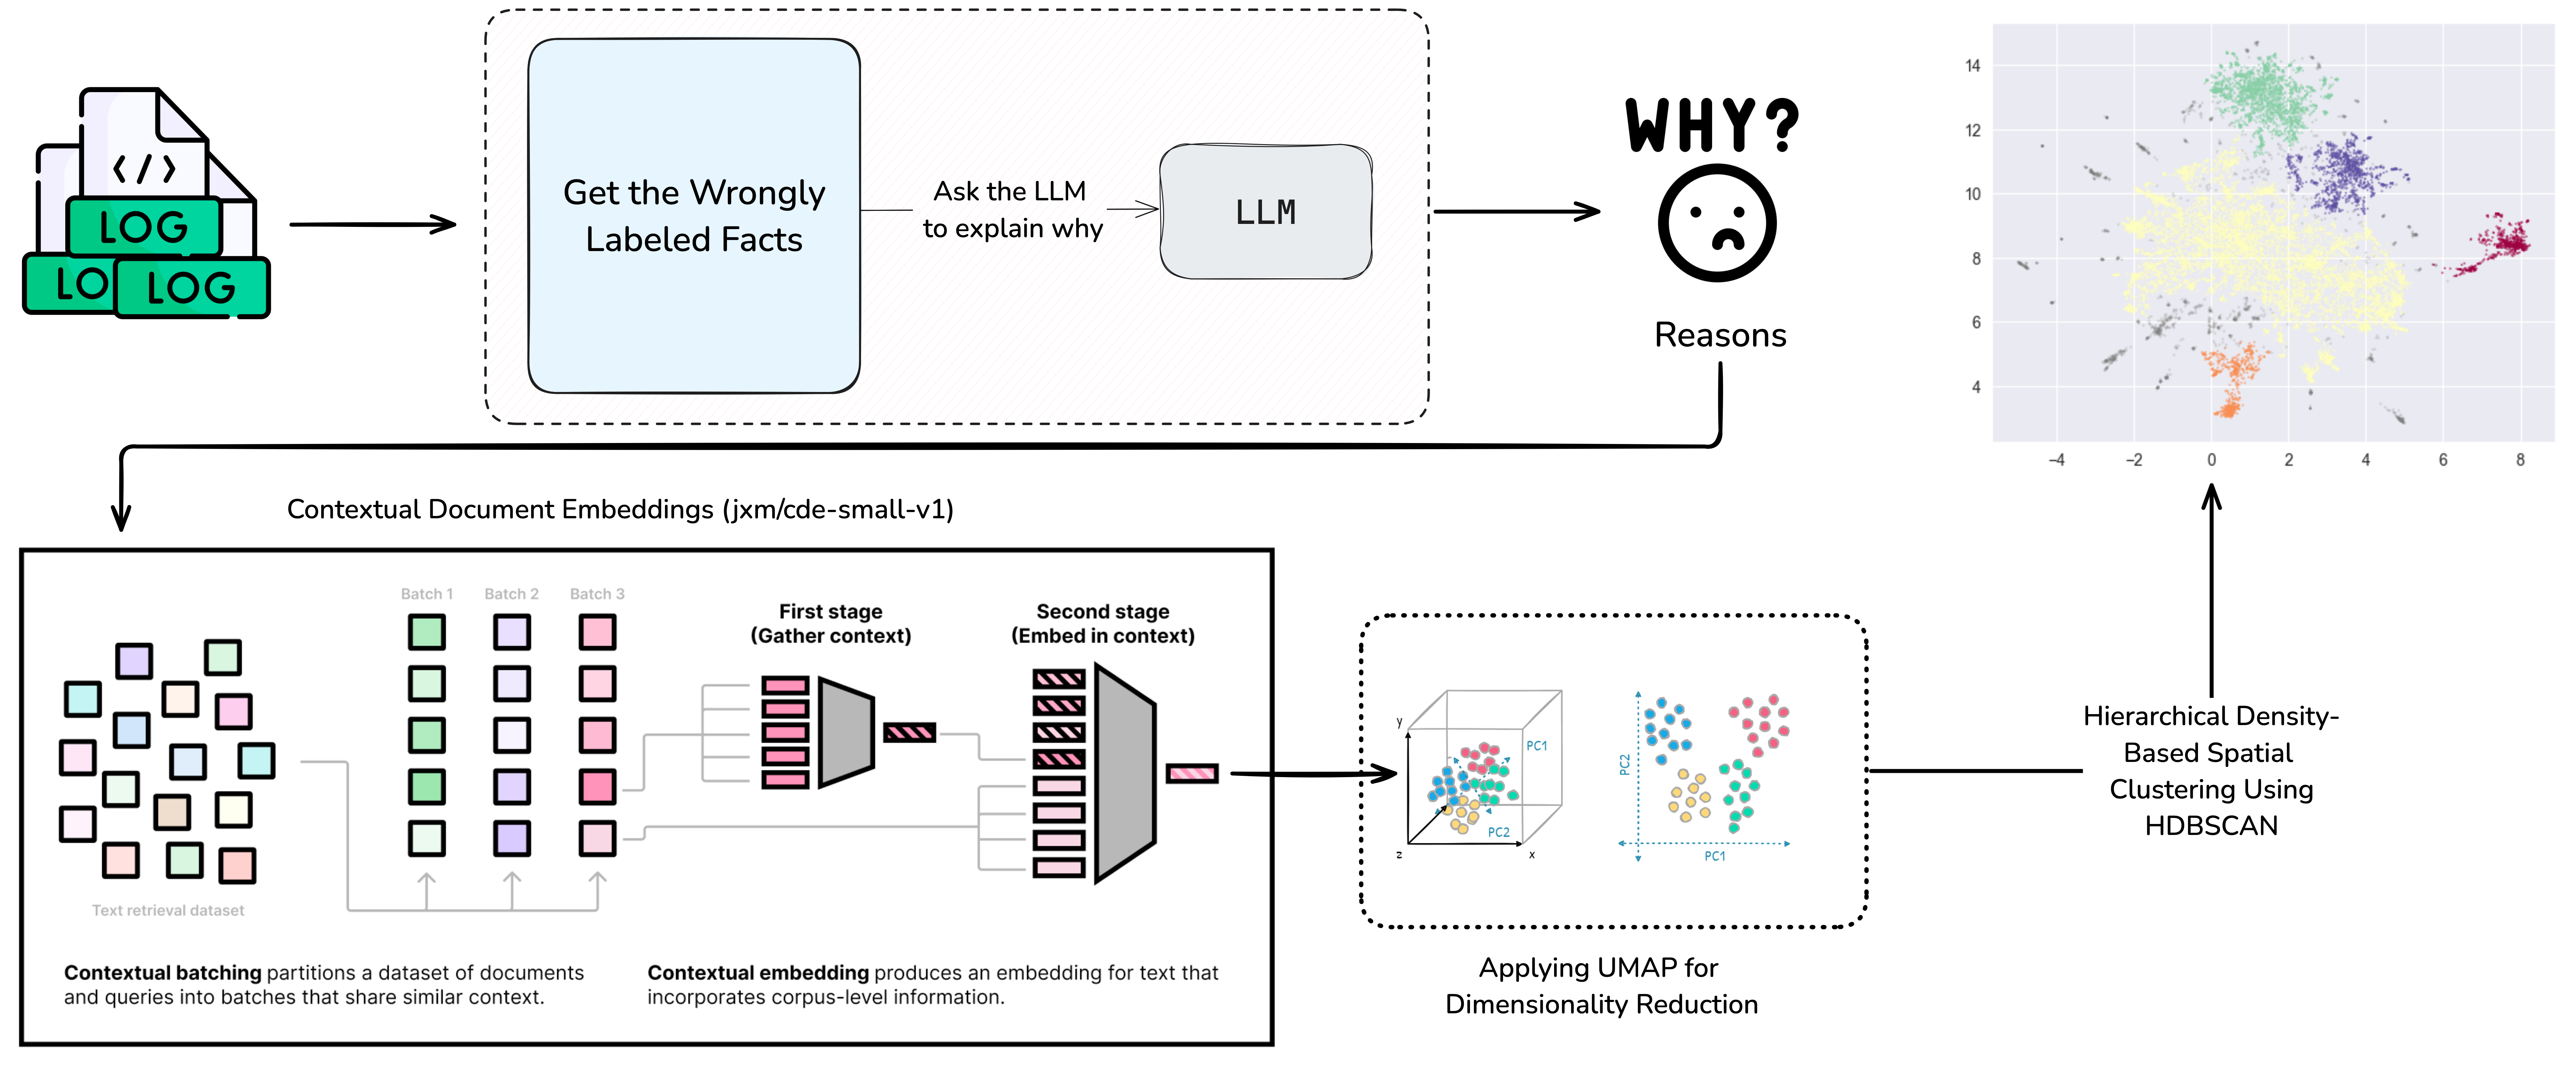
\includegraphics[width=\textwidth]{res/clustering}
    \end{minipage}
    \caption{Collecting logs and leveraging LLM-generated reasoning, combined with contextual document embeddings (jxm/cde-small-v1)~\cite{morris2024contextualdocumentembeddings}, to cluster errors using a hierarchical density-based spatial technique.}
    \label{fig:error-clustering-task}
\end{figure}

As depicted in Figure~\ref{fig:error-clustering-task}, our objective is to categorize errors by LLMs and text embedding model.
This approach helps reveal common error types and patterns by clustering explanations into distinct groups.
The process begins by gathering logs of incorrectly labeled data, referred to here as "wrongly labeled facts."
These logs are analyzed, and we then prompt an LLM to generate explanations, or "reasons," for each error.
This step provides context and may highlight underlying patterns or causes that contribute to these errors.
The prompt template used for this reasoning process is detailed in Appendix~\ref{sec:prompt-templates:reasoning}.
After obtaining explanations from the LLM, we use a specialized text embedding model named "jxm/cde-small-v1"~\footnote{\url{https://huggingface.co/jxm/cde-small-v1}}.
We selected cde-small-v1 because it is the highest-ranked small model (under 400 million parameters) on the MTEB leaderboard for text embedding models, as of October 1, 2024.
This model transforms each explanation into a contextualized embedding, capturing both semantic meaning and specific instruction-driven nuances for each error's context~\cite{morris2024contextualdocumentembeddings}.
Next, these embeddings undergo dimensionality reduction using Uniform Manifold Approximation and Projection (UMAP), a technique that projects high-dimensional data into two or three dimensions while preserving local and some global structure.
UMAP's visualization helps identify potential clusters or groupings of similar errors, making it easier to observe patterns that might be difficult to see in higher dimensions.
Once reduced in dimensionality, the embeddings are fed into Hierarchical Density-Based Spatial Clustering of Applications with Noise (HDBSCAN), a clustering algorithm well-suited for discovering clusters in data with varying density.
HDBSCAN clusters the error embeddings based on their density, identifying groups of similar errors and isolating outliers.
Following clustering, we identify some reasons from each dataset.
These representative reasons are then provided to an LLM to assign descriptive labels to each error category, which encapsulate the main types of errors across the dataset.

The labeling data for each cluster is as follows:
\begin{itemize}
    \item \textbf{UnLabeled:} The information or context provided does not contain the claimed details, such as references to specific individuals, places, or events that are purportedly associated with the topic.
    \item \textbf{Relationship Errors:} Errors arise from misstatements regarding relationships between people, such as marital status or religious affiliations that conflict with the provided details.
    \item \textbf{Role Attribution Errors:} Errors are due to incorrect associations of individuals with particular roles, places, or teams that do not match the details in the context.
    \item \textbf{Geographic/Nationality Errors:} This category includes errors related to locations, national affiliations, or settings that do not align with the context or provide contradictory information.
    \item \textbf{Genre/Classification Errors:} Misclassifications of films, genres, or roles are highlighted here, especially when certain works are wrongly associated with people, studios, or genres.
    \item \textbf{Identifier/Biographical Errors:} These errors involve incorrect identifiers or biographical details, such as award titles, label names, or authorship that don’t match the context.
\end{itemize}


\begin{table}[ht!]
    \noindent
    \caption{Dataset-wise error clustering based on LLM-generated reasoning, using Contextual Document Embeddings for embeddings, UMAP, and HDBSCAN.}
    \resizebox{\textwidth}{!}{
    \begin{threeparttable}
        \begin{tabular}{llcccccc||c}
            \toprule
            \textbf{Dataset}            & \textbf{Model} & \textbf{UnLabeled} & \textbf{Relationship} & \textbf{Role Errors} & \textbf{Geo Errors} & \textbf{Classification} & \textbf{Identifiers} & \textbf{Total}\tnote{*} \\
            \midrule
            \multirow{5}{*}{FactBench}  & Gemma2                             & 4    & 36    & 45    & 176  & 13     & 1     & 275 \\
                                        & Qwen2.5                            & 33   & 27    & 60    & 194  & 34     & 1     & 349 \\
                                        & Llama3.1                           & 38   & 44    & 73    & 295  & 38     & 3     & 491 \\
                                        & Mistral                            & 53   & 27    & 53    & 242  & 40     & 2     & 417 \\ \cline{2-9}
                                        & Unique. Ratio (\%)                 & 0.62 & 0.72  & 0.44  & 0.52 & 0.63   & 0.57  & 0.53 \\ \hline
            \multirow{5}{*}{YAGO}       & Gemma2                             & 6        & 134   & 0   & 14      & 51    & 2     & 207   \\
                                        & Qwen2.5                            & 7        & 109   & 0   & 13      & 63    & 2     & 194   \\
                                        & Llama3.1                           & 8        & 98    & 0   & 19      & 104   & 2     & 231   \\
                                        & Mistral                            & 7        & 54    & 0   & 10      & 34    & 3     & 108   \\ \cline{2-9}
                                        & Unique. Ratio (\%)                 & 0.35     & 0.52  & --   & 0.46    & 0.51  & 0.33  & 0.50  \\ \hline
            \multirow{5}{*}{DBpedia}    & Gemma2                             & 353      & 22    & 98  & 1729    & 459   & 299   & 2960  \\
                                        & Qwen2.5                            & 339      & 19    & 91  & 1525    & 357   & 237   & 2568 \\
                                        & Llama3.1                           & 382      & 28    & 109 & 2172    & 509   & 318   & 3518 \\
                                        & Mistral                            & 325      & 20    & 94  & 1487    & 438   & 241   & 2605 \\ \cline{2-9}
                                        & Unique. Ratio (\%)                 & 0.41     & 0.43  & 0.44 & 0.42   & 0.42  & 0.40  & 0.41 \\
            \bottomrule
        \end{tabular}
    \begin{tablenotes}
         \item[*] Some errors may not be included in this analysis because we did not receive any responses for them. While we classify these as incorrect predictions, they are not considered in the error analysis section.
    \end{tablenotes}
    \end{threeparttable}}
    \label{tab:error_results-full-wo-category-all-datasets}
\end{table}

\begin{figure}[ht!]
    \centering
    \begin{minipage}[b]{\textwidth}
        \centering
        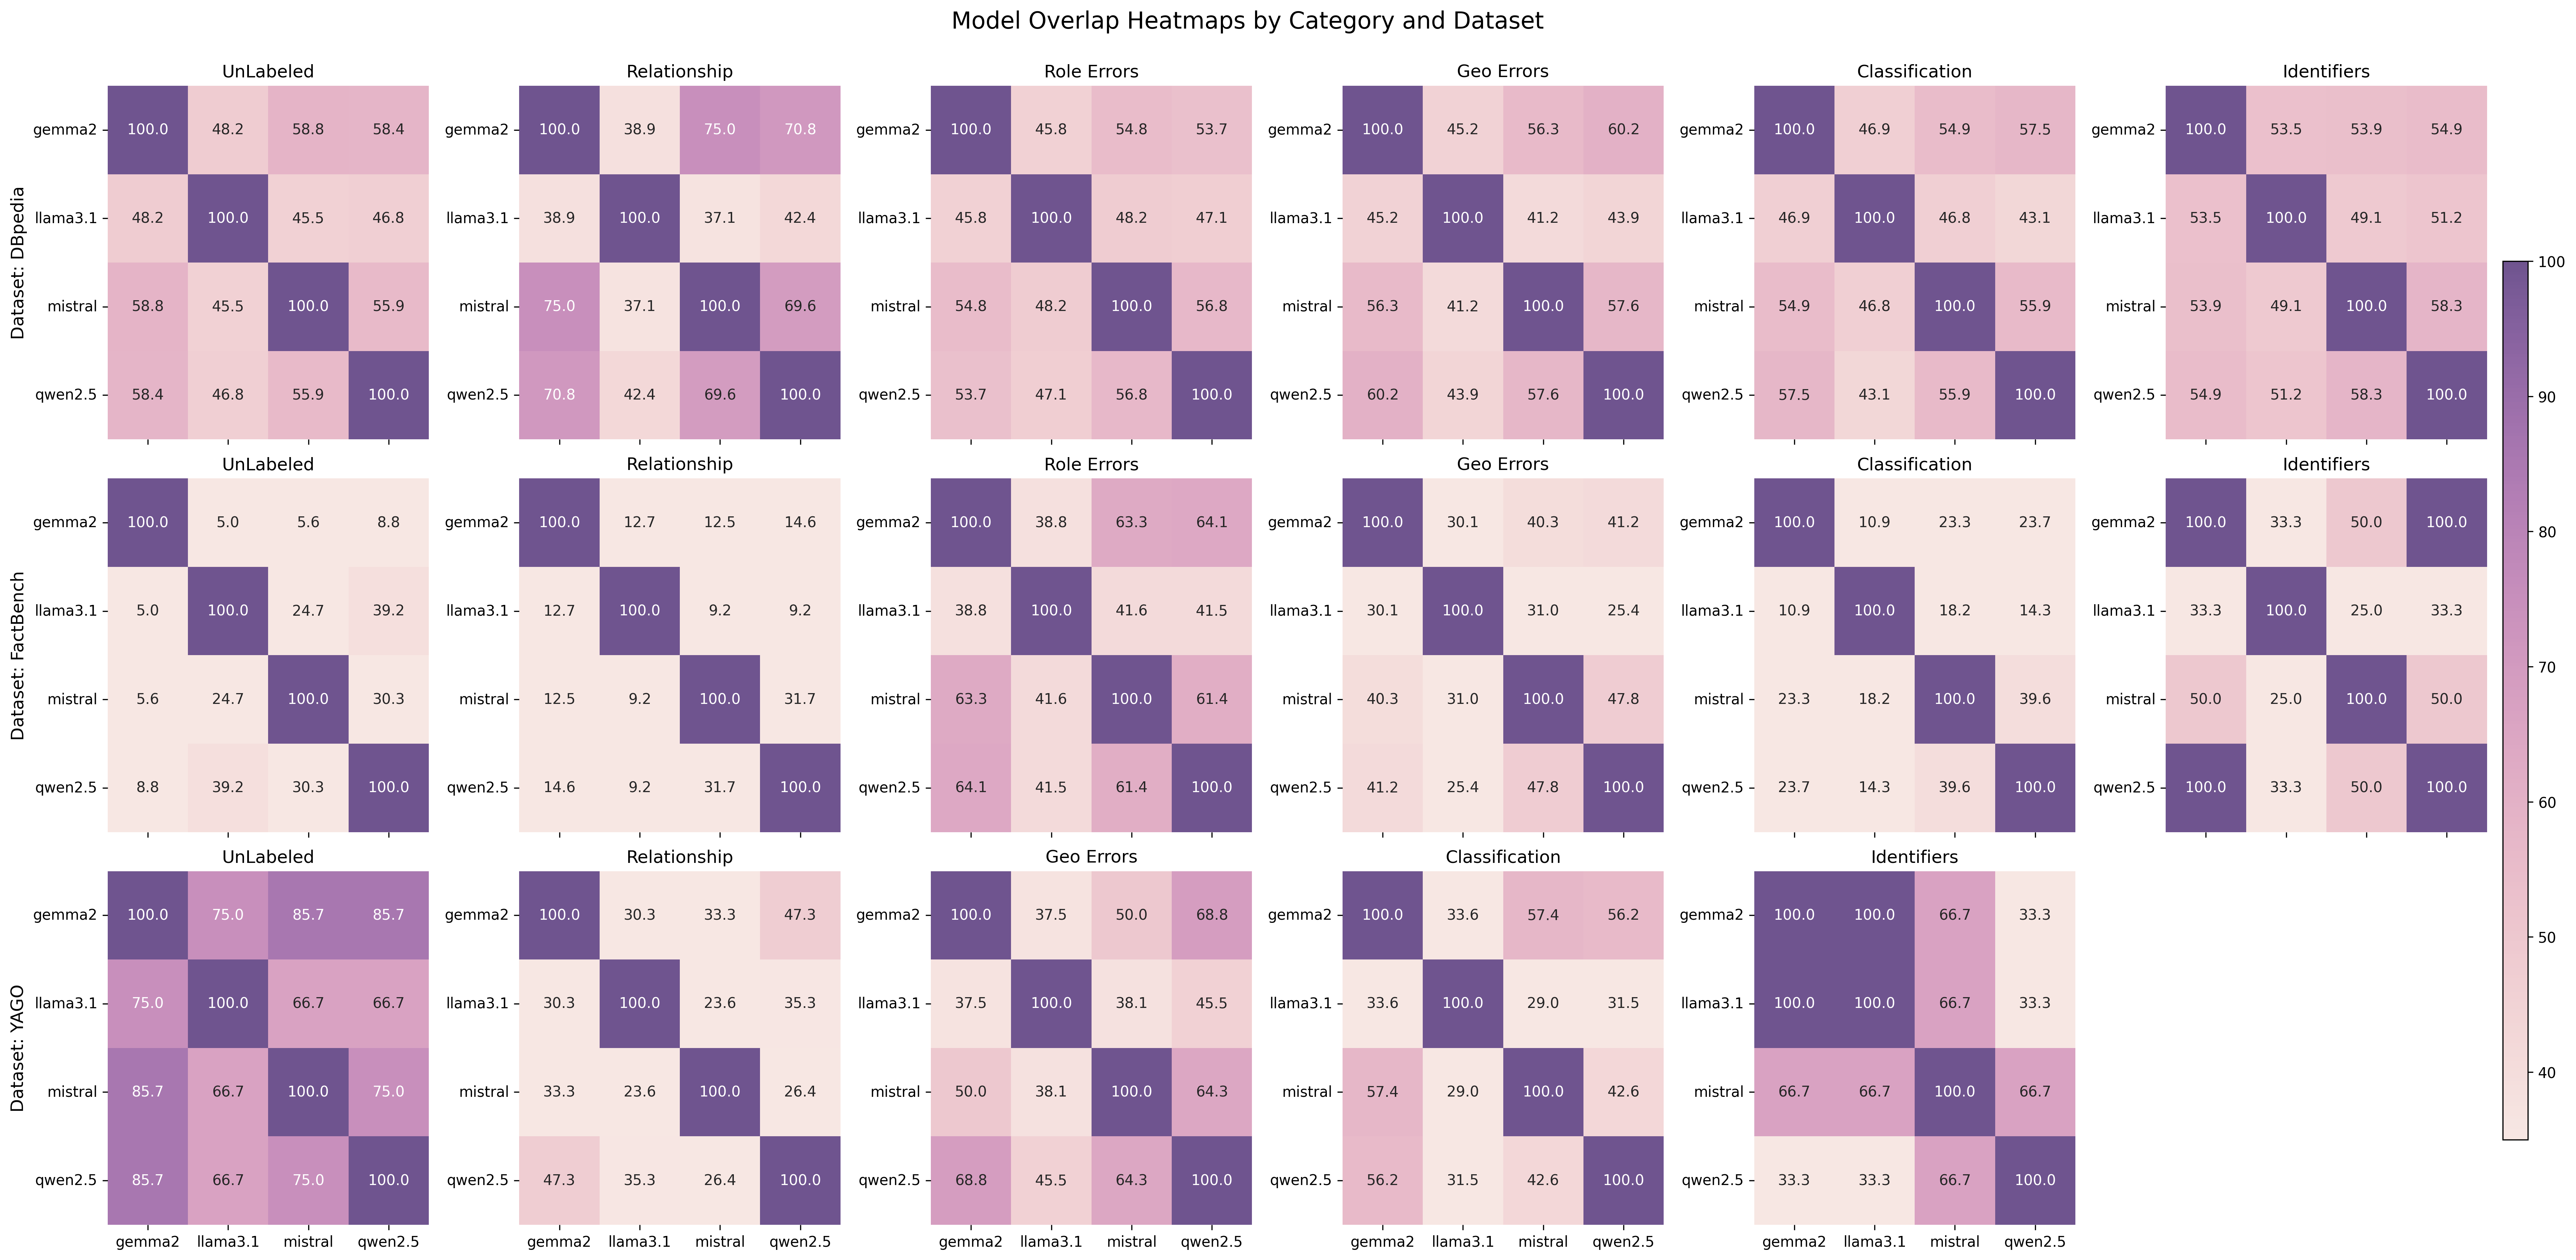
\includegraphics[width=\textwidth]{res/overlap_heatmaps_by_dataset}
    \end{minipage}
    \caption{Model overlap heatmaps by category and dataset. Each cell shows the percentage overlap in errors between model pairs. Matrices are organized by error category (UnLabeled, Relationship, Role Errors, etc.) and dataset (DBpedia, FactBench, YAGO), revealing patterns in how models agree or disagree when making verification errors.}
    \label{fig:overlap_heatmaps_by_dataset}
\end{figure}

The heatmaps in Figure~\ref{fig:overlap_heatmaps_by_dataset} visualize the overlap in error patterns between different models across error categories and datasets.
The overlap matrices reveal distinct patterns of agreement and disagreement between models when making errors, with darker colors indicating higher overlap percentages.
For \textit{DBpedia}, we observe moderate to high overlap (45-75\%) between models across most error categories, suggesting similar challenges in handling complex factual relationships.
The \textit{FactBench} dataset shows lower overlap percentages (30-40\% typical), indicating more independent error patterns between models.
\textit{YAGO} exhibits variable overlap, with particularly high agreement in unlabeled errors (75-85\% overlap) but lower overlap in relationship errors (23-35\%).
These patterns suggest that while models often struggle with similar types of facts, they also make distinct errors, supporting the value of ensemble approaches.
The lower overlap in \textit{FactBench} errors particularly validates our multi-model verification strategy.

\begin{figure}[ht!]
    \centering
    \begin{minipage}[b]{0.42\textwidth}
        \centering
        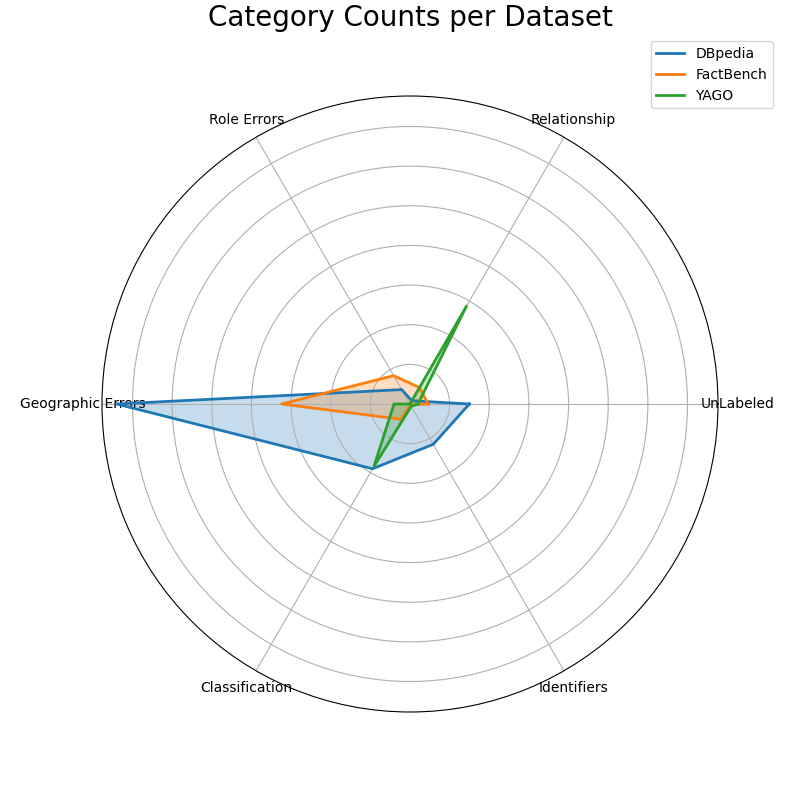
\includegraphics[width=\textwidth]{res/radarChart-normalized}
        \caption{Normalized distribution of error clusters across datasets.}
        \label{fig:normalized_distribution_of_error_clusters}
    \end{minipage}
    \hspace{0.05\textwidth} % Space between the images
    \begin{minipage}[b]{0.42\textwidth}
        \centering
        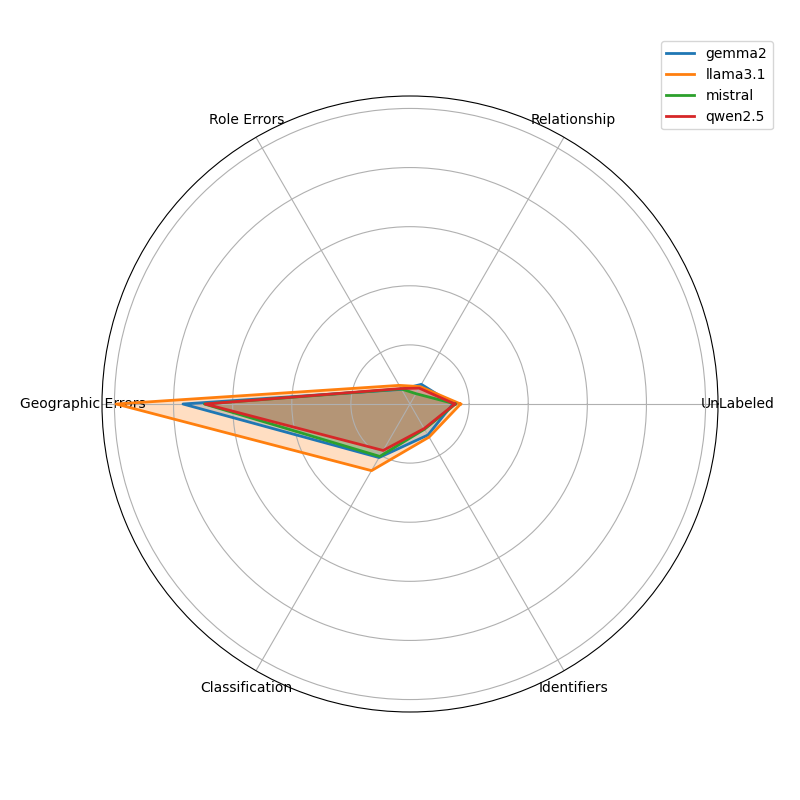
\includegraphics[width=\textwidth]{res/radarChart-normalized-llms}
        \caption{Distribution of error clusters across selected LLMs.}
        \label{fig:distribution_of_error_clusters}
    \end{minipage}
\end{figure}

\begin{figure}[ht!]
    \centering
    \begin{minipage}[b]{0.42\textwidth}
        \centering
        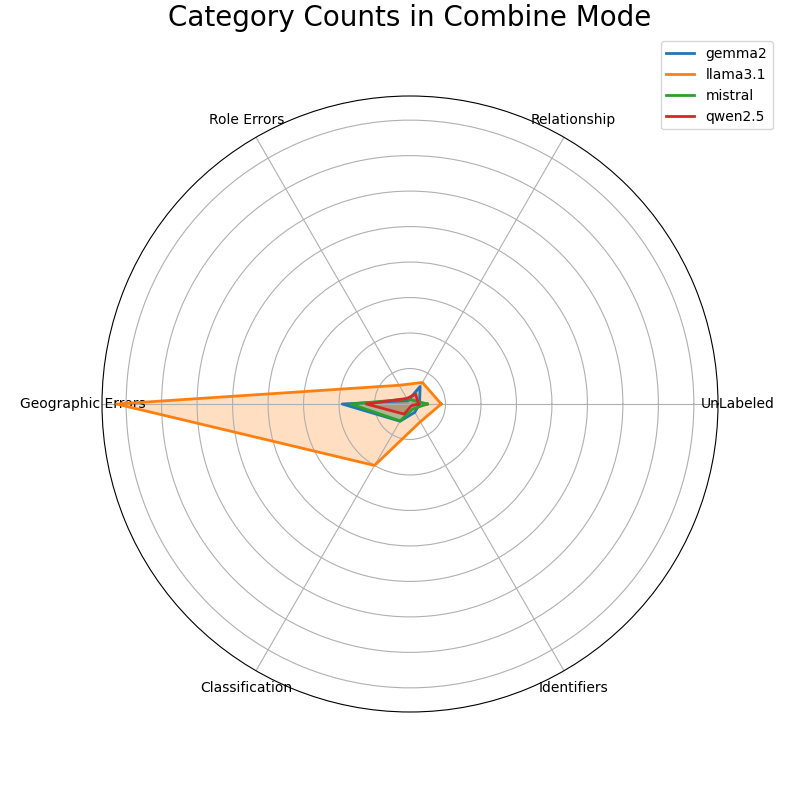
\includegraphics[width=\textwidth]{res/radarChart-normalized-llms-1}
    \end{minipage}
    \hspace{0.05\textwidth} % Space between the images
    \begin{minipage}[b]{0.42\textwidth}
        \centering
        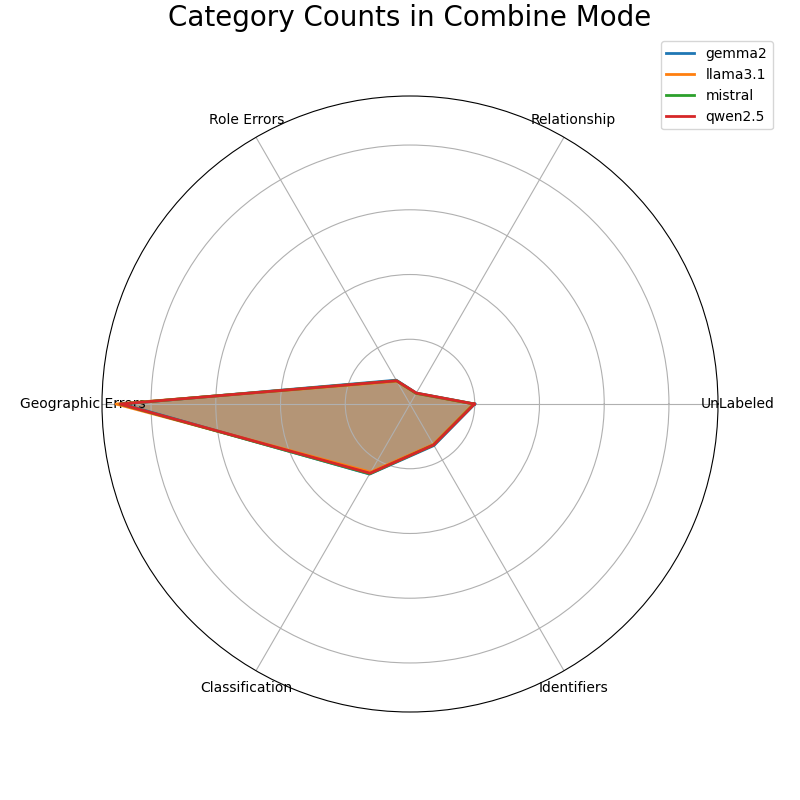
\includegraphics[width=\textwidth]{res/radarChart-normalized-llms-4}
    \end{minipage}
    \caption{Distribution of tendency to be wrong across gemma2, qwen2.5, LLama3.1 and mistral models. The right chart illustrates the distribution of fully incorrect predictions (4/4) detailing the instances where all predictions made by the models were incorrect. The left chart depicts the distribution of just one wrong predictions (1/4).}
    \label{fig:distribution_of_error_clusters_1_4}
\end{figure}

Results from Table~\ref{tab:error_results-full-wo-category-all-datasets} alongside Figures~\ref{fig:normalized_distribution_of_error_clusters}, ~\ref{fig:distribution_of_error_clusters}, and~\ref{fig:distribution_of_error_clusters_1_4} highlight both common challenges and model-specific characteristics in fact validation performance.

Geographic and nationality-related errors emerged as the predominant challenge, accounting for 56.9\% of total errors across all models and datasets.
This pattern was particularly pronounced in the \textit{DBpedia} dataset, where geographic errors constituted 58.5\% of all errors, suggesting a systematic challenge in processing and validating location-based information.
This pervasive difficulty across all models indicates a fundamental challenge in handling geographic relationships and facts.

The analysis of dataset-specific patterns revealed distinct characteristics and challenges.
The \textit{DBpedia} dataset proved to be the most challenging, generating the highest error count and showing particular vulnerability to geographic and classification errors.
In contrast, the \textit{FactBench} dataset demonstrated a more balanced distribution of errors across categories, though still showing a predominance of geographic errors.
The \textit{YAGO} dataset exhibited a unique pattern, with relationship errors being the most frequent, followed by classification errors, and notably showing no role attribution errors a distinctive characteristic that sets it apart from other datasets.

When examining model-specific performance, \textit{LLama3.1} consistently generated the highest error counts across datasets, showing particular vulnerability to geographic errors in the \textit{DBpedia} dataset and elevated classification errors compared to other models.
\textit{Mistral}, on the other hand, demonstrated stronger overall performance, particularly in the \textit{YAGO} dataset.
\textit{Gemma2} and \textit{Qwen2.5} showed similar error patterns and counts, positioning themselves between \textit{LLama3.1} and \textit{Mistral} in terms of performance.

The hierarchical distribution of error types shows a consistent pattern across models.
This consistency in error distribution suggests that these challenges are inherent to the task rather than model-specific limitations.

Despite varying error counts, models maintained similar error distribution patterns within each dataset, indicating that these challenges are systematic rather than model-specific.
The analysis suggests several critical areas for future development in LLM fact validation capabilities.
Primary attention should be directed toward enhancing geographic and location-based reasoning capabilities, given their dominant role in error generation.
Additionally, improving classification tasks and the handling of insufficient context or ambiguous information could significantly enhance overall performance.
The consistent patterns across models suggest that these improvements would benefit the field broadly rather than being model-specific enhancements.

\subsection{DBpedia Analysis in Depth}\label{subsec:db}
Since \textit{DBpedia} proved to be the most challenging dataset in our evaluation, we performed a deeper analysis based on the dataset stratification established by Marchesin et al.~\cite{Marchesin_Silvello_Alonso_2024}.
Each knowledge graph triple was assigned to one of seven partitions, numbered 1--7, where partition 1 represents the least popular/common knowledge and partition 7 represents the most popular/common knowledge.
This stratification helps us understand how our verification system performs across different levels of fact popularity and complexity within \textit{DBpedia}.
The analysis can reveal whether the system's accuracy varies between common, well-documented facts versus more obscure or specialized knowledge.
This insight is valuable for identifying areas where the system needs improvement and understanding its real-world applicability across different types of knowledge.

\begin{table}[ht!]
    \noindent
    \caption{Partition-wise evaluation results of the proposed system and candidate LLMs over the DBpedia dataset.}
    \resizebox{\textwidth}{!}{
        \begin{tabular}{lcccccccccccccccc}
            \toprule
            & \multirow{2}{*}{\textbf{Weight}} & \multirow{2}{*}{\textbf{Size}} & \multicolumn{2}{c}{\textbf{Gemma2}}       & \multicolumn{2}{c}{\textbf{Qwen2.5}}          & \multicolumn{2}{c}{\textbf{Llama3.1}}         & \multicolumn{2}{c}{\textbf{Mistral}}     & \multicolumn{2}{c}{\textbf{Qwen2.5:14b}}         & \multicolumn{2}{c}{\textbf{Llama3.1:70b}} \\ \cmidrule(lr){4-5} \cmidrule(lr){6-7} \cmidrule(lr){8-9} \cmidrule(lr){10-11} \cmidrule(lr){12-13} \cmidrule(lr){14-15}
            & & & \textbf{Acc}         & \textbf{F1}       & \textbf{Acc}          & \textbf{F1}           & \textbf{Acc}            & \textbf{F1}         & \textbf{Acc}             & \textbf{F1}     & \textbf{Acc}               & \textbf{F1}         & \textbf{Acc}                & \textbf{F1} \\
            \midrule
            Stratum 1    &  0.9120   & 2223 & 0.672                & 0.773             & 0.708                 & 0.804                 & 0.600                   & 0.712               & 0.710                   & 0.806          & 0.688                      & 0.786               & 0.700                       & 0.797       \\
            Stratum 2    &  0.0616   & 1695 & 0.697                & 0.796             & 0.720                 & 0.816                 & 0.627                   & 0.738               & 0.726                   & 0.820          & 0.711                      & 0.807               & 0.720                       & 0.814       \\
            Stratum 3    &  0.0177   & 1588 & 0.689                & 0.791             & 0.736                 & 0.828                 & 0.632                   & 0.743               & 0.719                   & 0.819          & 0.708                      & 0.806               & 0.719                       & 0.815       \\
            Stratum 4    &  0.0044   & 1327 & 0.689                & 0.797             & 0.737                 & 0.835                 & 0.628                   & 0.747               & 0.709                   & 0.815          & 0.706                      & 0.811               & 0.714                       & 0.817       \\
            Stratum 5    &  0.0029   & 1058 & 0.666                & 0.780             & 0.705                 & 0.813                 & 0.638                   & 0.758               & 0.724                   & 0.826          & 0.690                      & 0.800               & 0.695                       & 0.804       \\
            Stratum 6    &  0.0010   & 814  & 0.692                & 0.800             & 0.719                 & 0.822                 & 0.614                   & 0.739               & 0.733                   & 0.833          & 0.709                      & 0.813               & 0.708                       & 0.812       \\
            Stratum 7    &  0.0001   & 629  & 0.671                & 0.776             & 0.779                 & 0.864                 & 0.650                   & 0.762               & 0.754                   & 0.848          & 0.731                      & 0.826               & 0.747                       & 0.838       \\
            \bottomrule
        \end{tabular}}
    \label{tab:evaluation_results-partition-wise-dbpedia}
\end{table}

The weights declared in Table~\ref{tab:evaluation_results-partition-wise-dbpedia} are gathered by Marchesin et al.~\cite{Marchesin_Silvello_Alonso_2024}, stratum 1 contains the vast majority of the triplets in DBpedia.
This makes sense because stratum 1 represents the lowest-utility facts - those that are rarely used in queries.

\begin{figure}[ht!]
    \centering
    \begin{minipage}[b]{\textwidth}
        \centering
        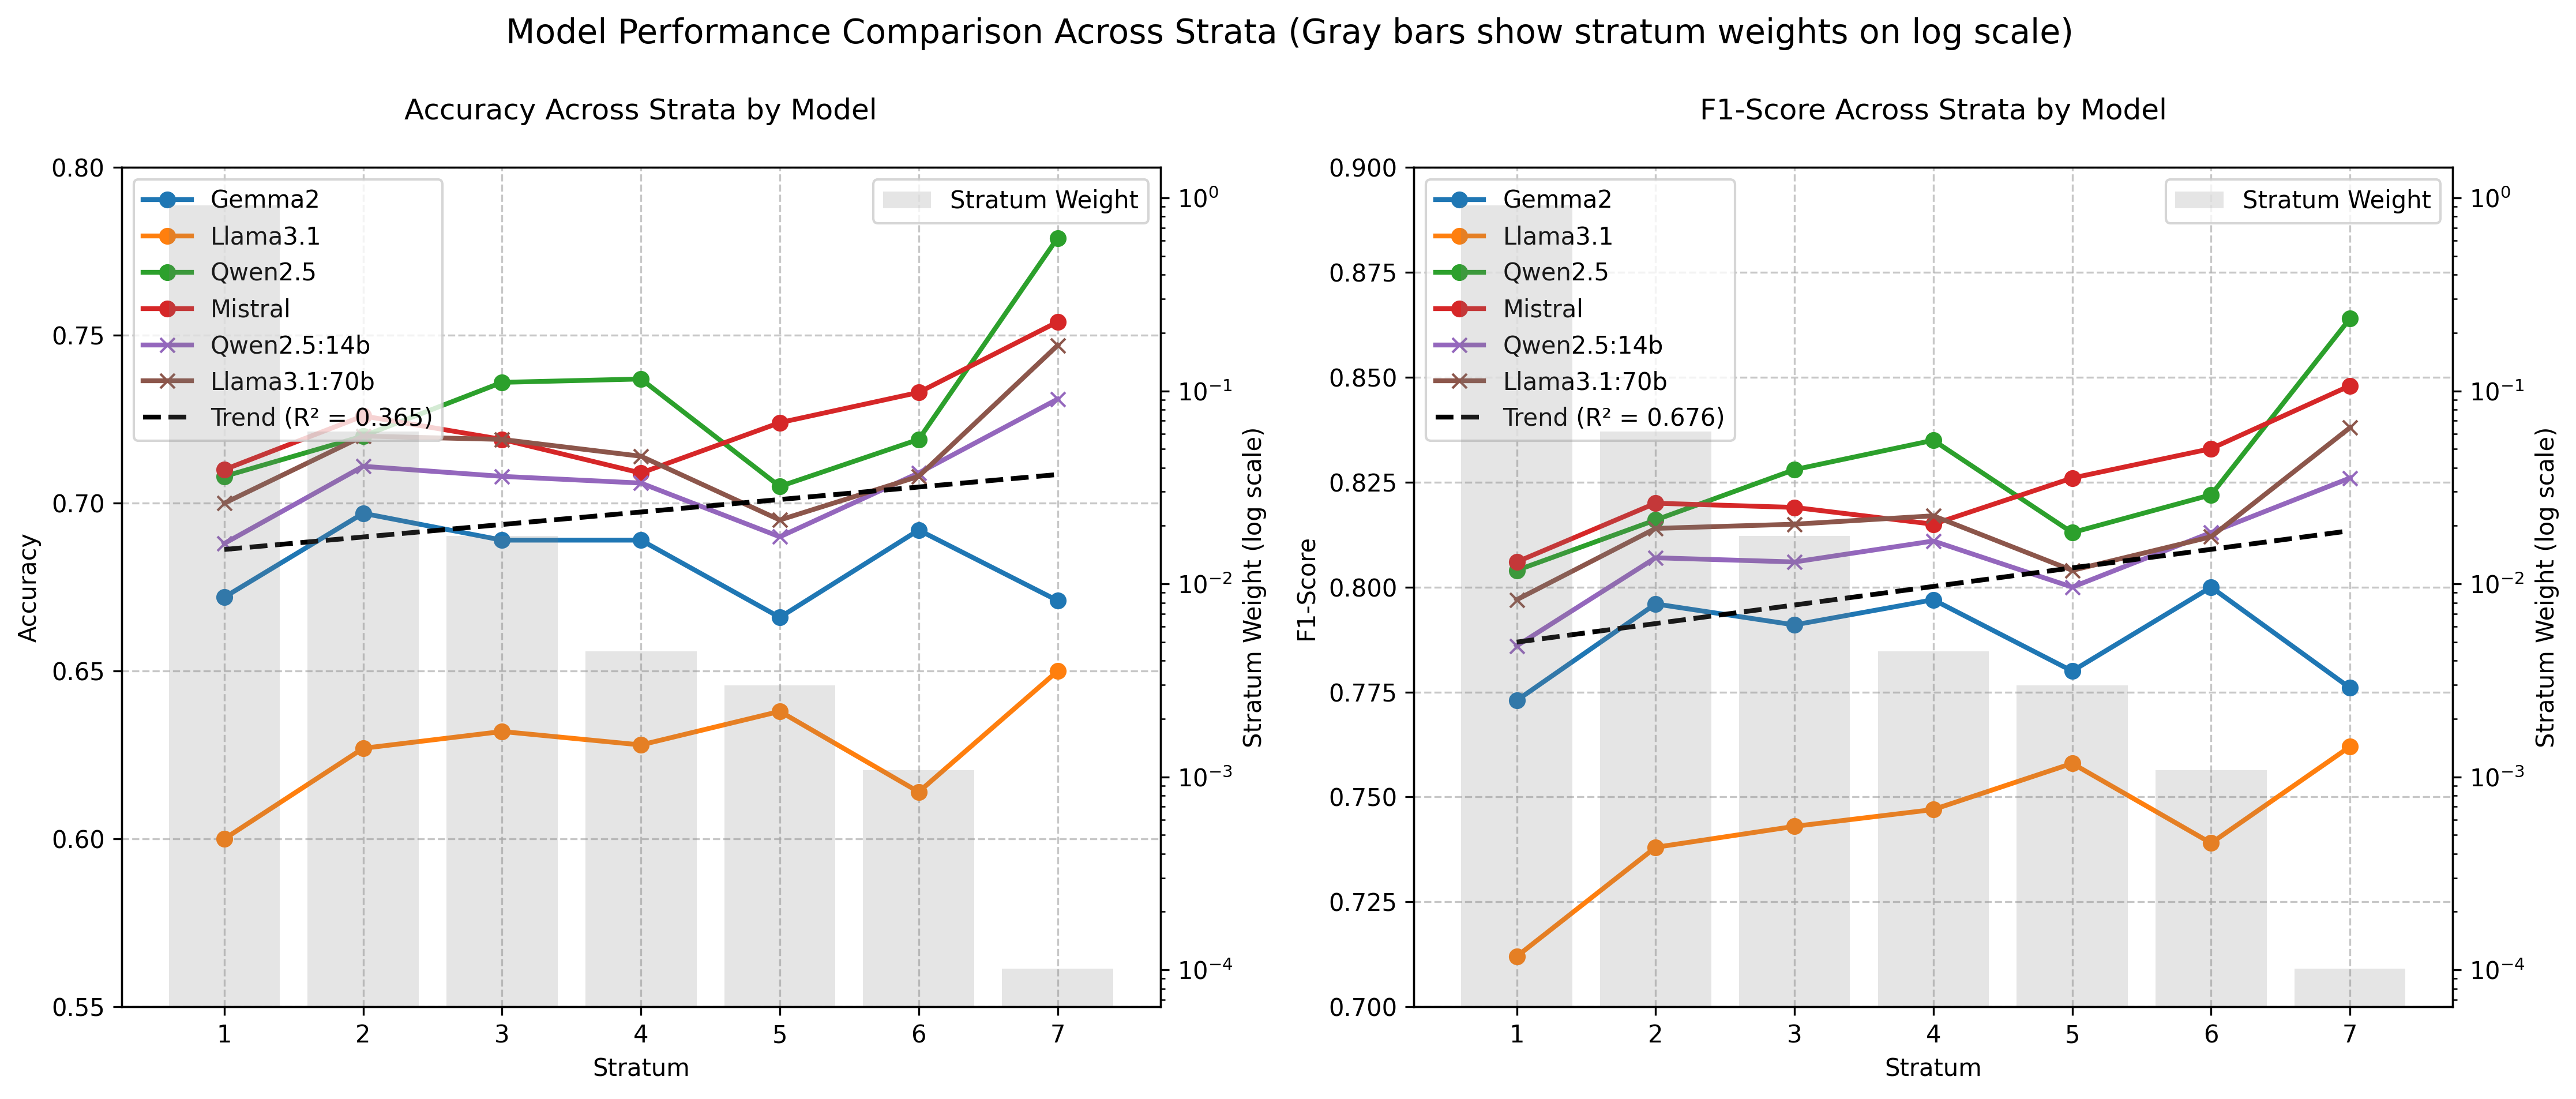
\includegraphics[width=\textwidth]{res/F1_ACC_Analysis_Across_Stratum}
    \end{minipage}
    \caption{Partition-wise model performance comparison: Accuracy and F1-scores for knowledge graph fact verification on DBpedia dataset. Gray bars indicate stratum weights (log scale).}
    \label{fig:F1_ACC_Analysis_Across_Stratum}
\end{figure}

Table~\ref{tab:evaluation_results-partition-wise-dbpedia} and Figure~\ref{fig:F1_ACC_Analysis_Across_Stratum}, demonstrate that the models have a clear trend of improved performance on more common knowledge.
\textit{Qwen2.5} exhibits particularly strong performance, with accuracy increasing from 0.708 in Stratum 1 to 0.779 in Stratum 7, and F1-scores following a similar upward trajectory.
This suggests that the model benefits from the richer context and more consistent representation of popular facts in the knowledge base.

The performance disparity between lower and higher strata highlights a common challenge in knowledge graph verification: the system's reliability varies with fact popularity.
This insight is particularly valuable for real-world applications, where handling both common and specialized knowledge is crucial.

Building on our previous analysis of \textit{DBpedia} results, we conducted a stratum-wise error analysis to better understand how error distributions vary across different data partitions.
Our analysis of error patterns across knowledge strata showed in Figure~\ref{fig:error_model-comparison_partition-wise} declares distinct performance characteristics among the four LLMs.
The models demonstrated varying levels of effectiveness in handling knowledge from different popularity strata, with error rates showing notable patterns across the commonality spectrum.

\begin{figure}[ht!]
    \centering
    \begin{minipage}[b]{\textwidth}
        \centering
        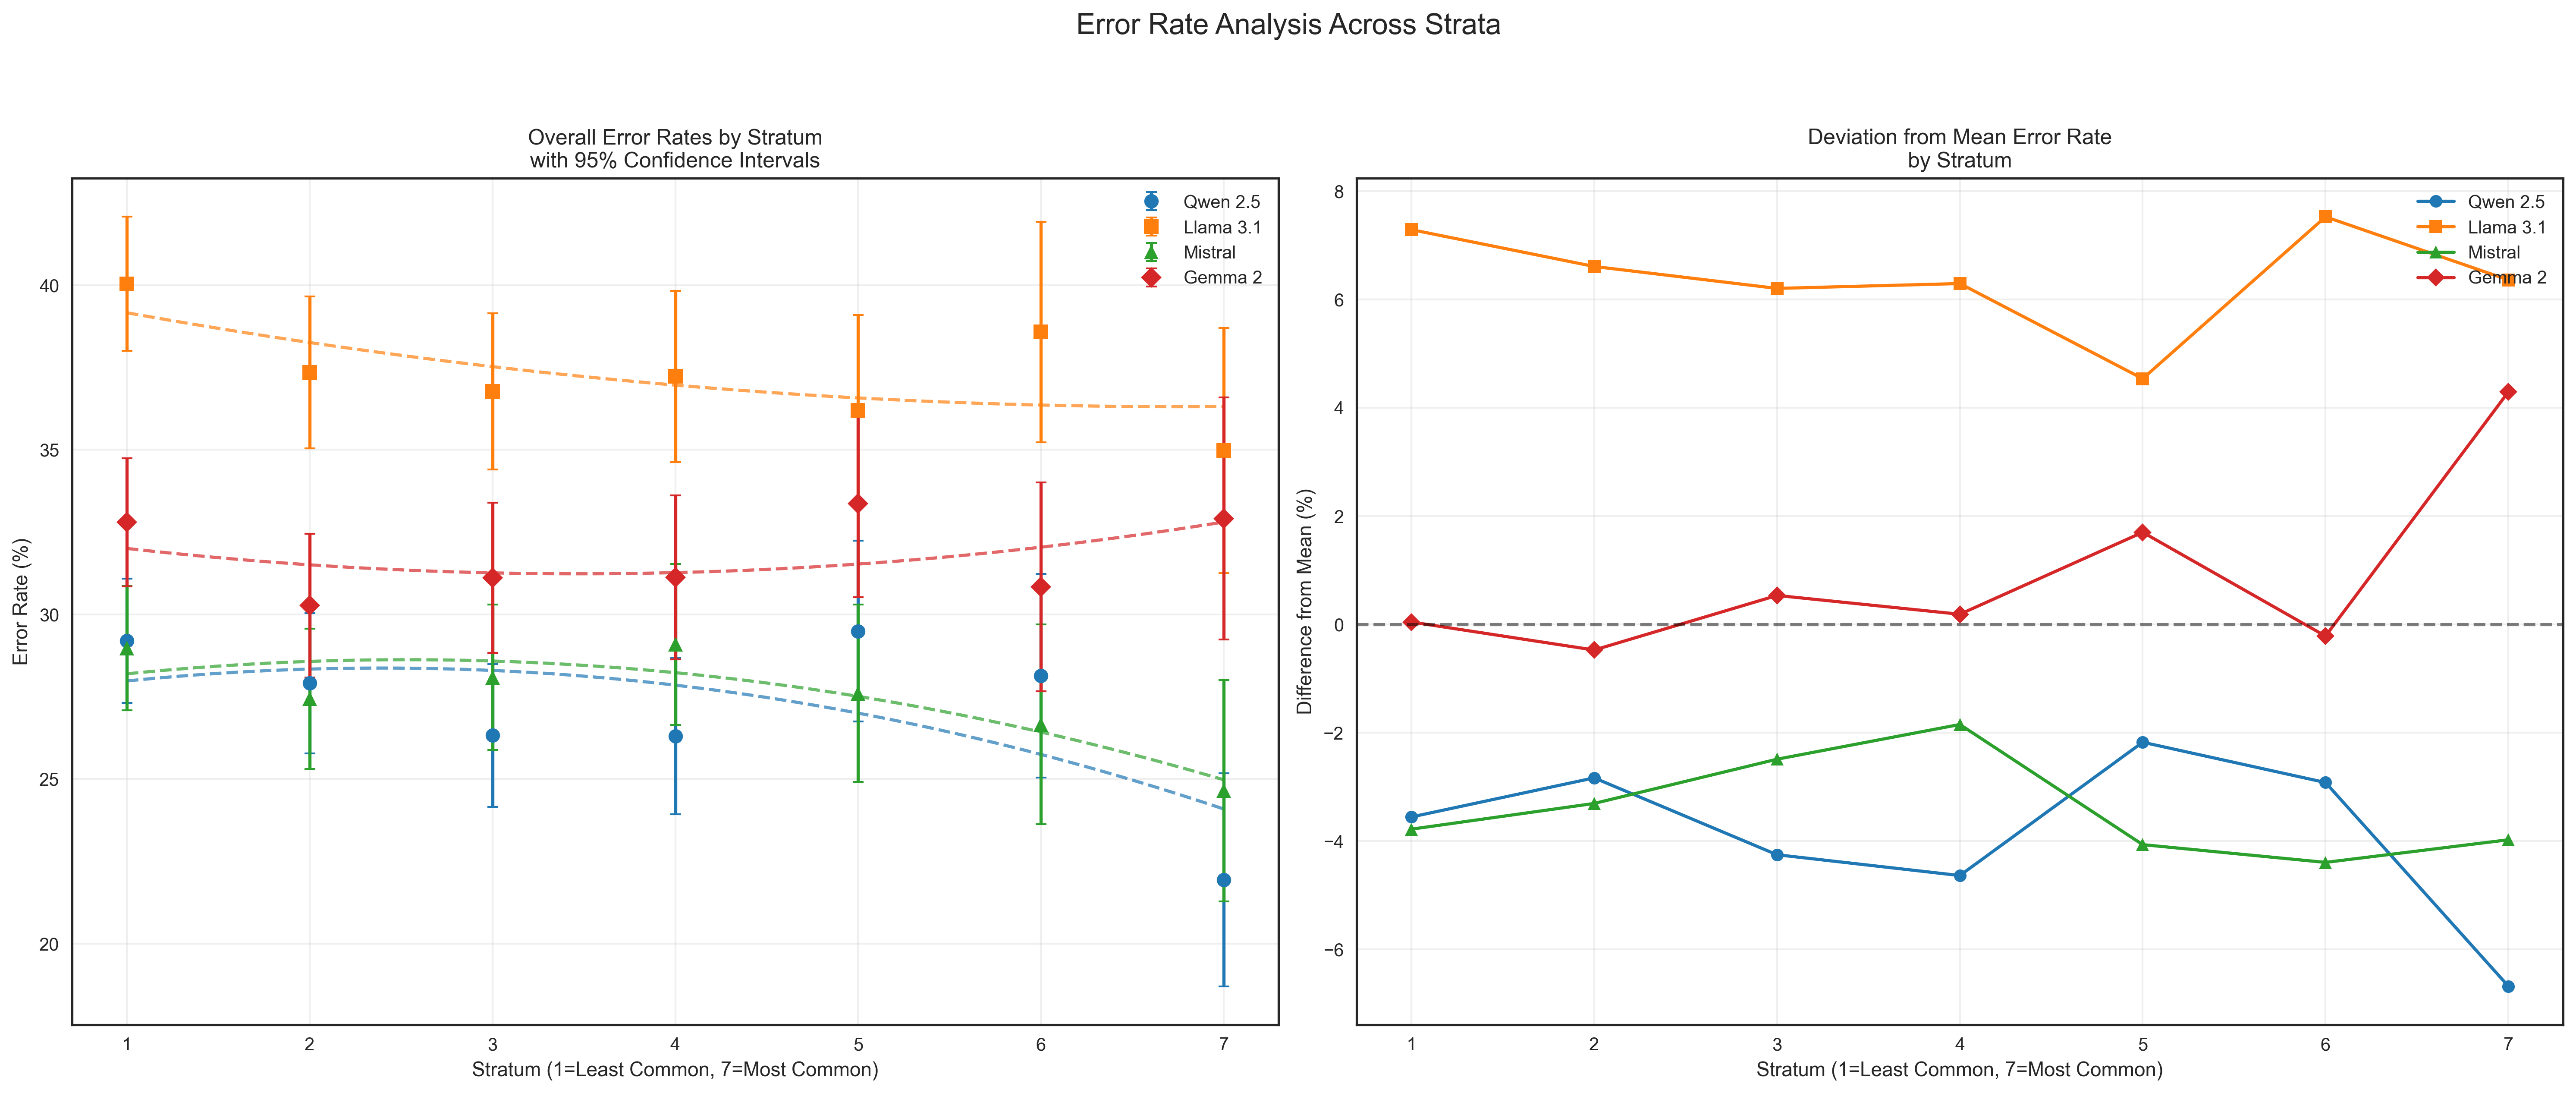
\includegraphics[width=\textwidth]{res/error_rates_analysis}
    \end{minipage}
    \caption{Error distribution analysis across different language models and frequency strata.}
    \label{fig:error_model-comparison_partition-wise}
\end{figure}

\textit{Llama3.1} exhibited the highest overall error rate (37.31\% ± 1.51\%), significantly exceeding other models' error rates.
Despite its higher error rate, \textit{Llama3.1} maintained relatively consistent performance across strata (range: 34.98\% - 40.04\%), suggesting uniform handling of both common and rare knowledge.
The model showed a slight negative correlation with stratum number (r=-0.628, p=0.1309), indicating a modest tendency to perform better with more common knowledge, though this trend was not statistically significant.

In contrast, \textit{Qwen2.5} and \textit{Mistral} demonstrated notably lower error rates (27.04\% ± 2.38\% and 27.50\% ± 1.41\% respectively), with \textit{Mistral} showing the most pronounced negative correlation with stratum number (r=-0.761, p=0.0470).
This statistically significant correlation indicates that \textit{Mistral's} performance improves substantially as knowledge becomes more common.
\textit{Qwen2.5} showed the widest range of error rates (21.94\% - 29.49\%), suggesting more variable performance across different knowledge types.

\textit{Gemma2} maintained an intermediate position with a mean error rate of 31.77\% ± 1.13\% and showed the most stable performance across strata (range: 30.27\% - 33.36\%).
Uniquely among the models, \textit{Gemma2} exhibited a slight positive correlation with stratum number (r=0.237, p=0.6083), though this trend was not statistically significant.
In general, it has the most uniform error distribution across strata.

\begin{figure}[ht!]
    \centering
    \begin{minipage}[b]{\textwidth}
        \centering
        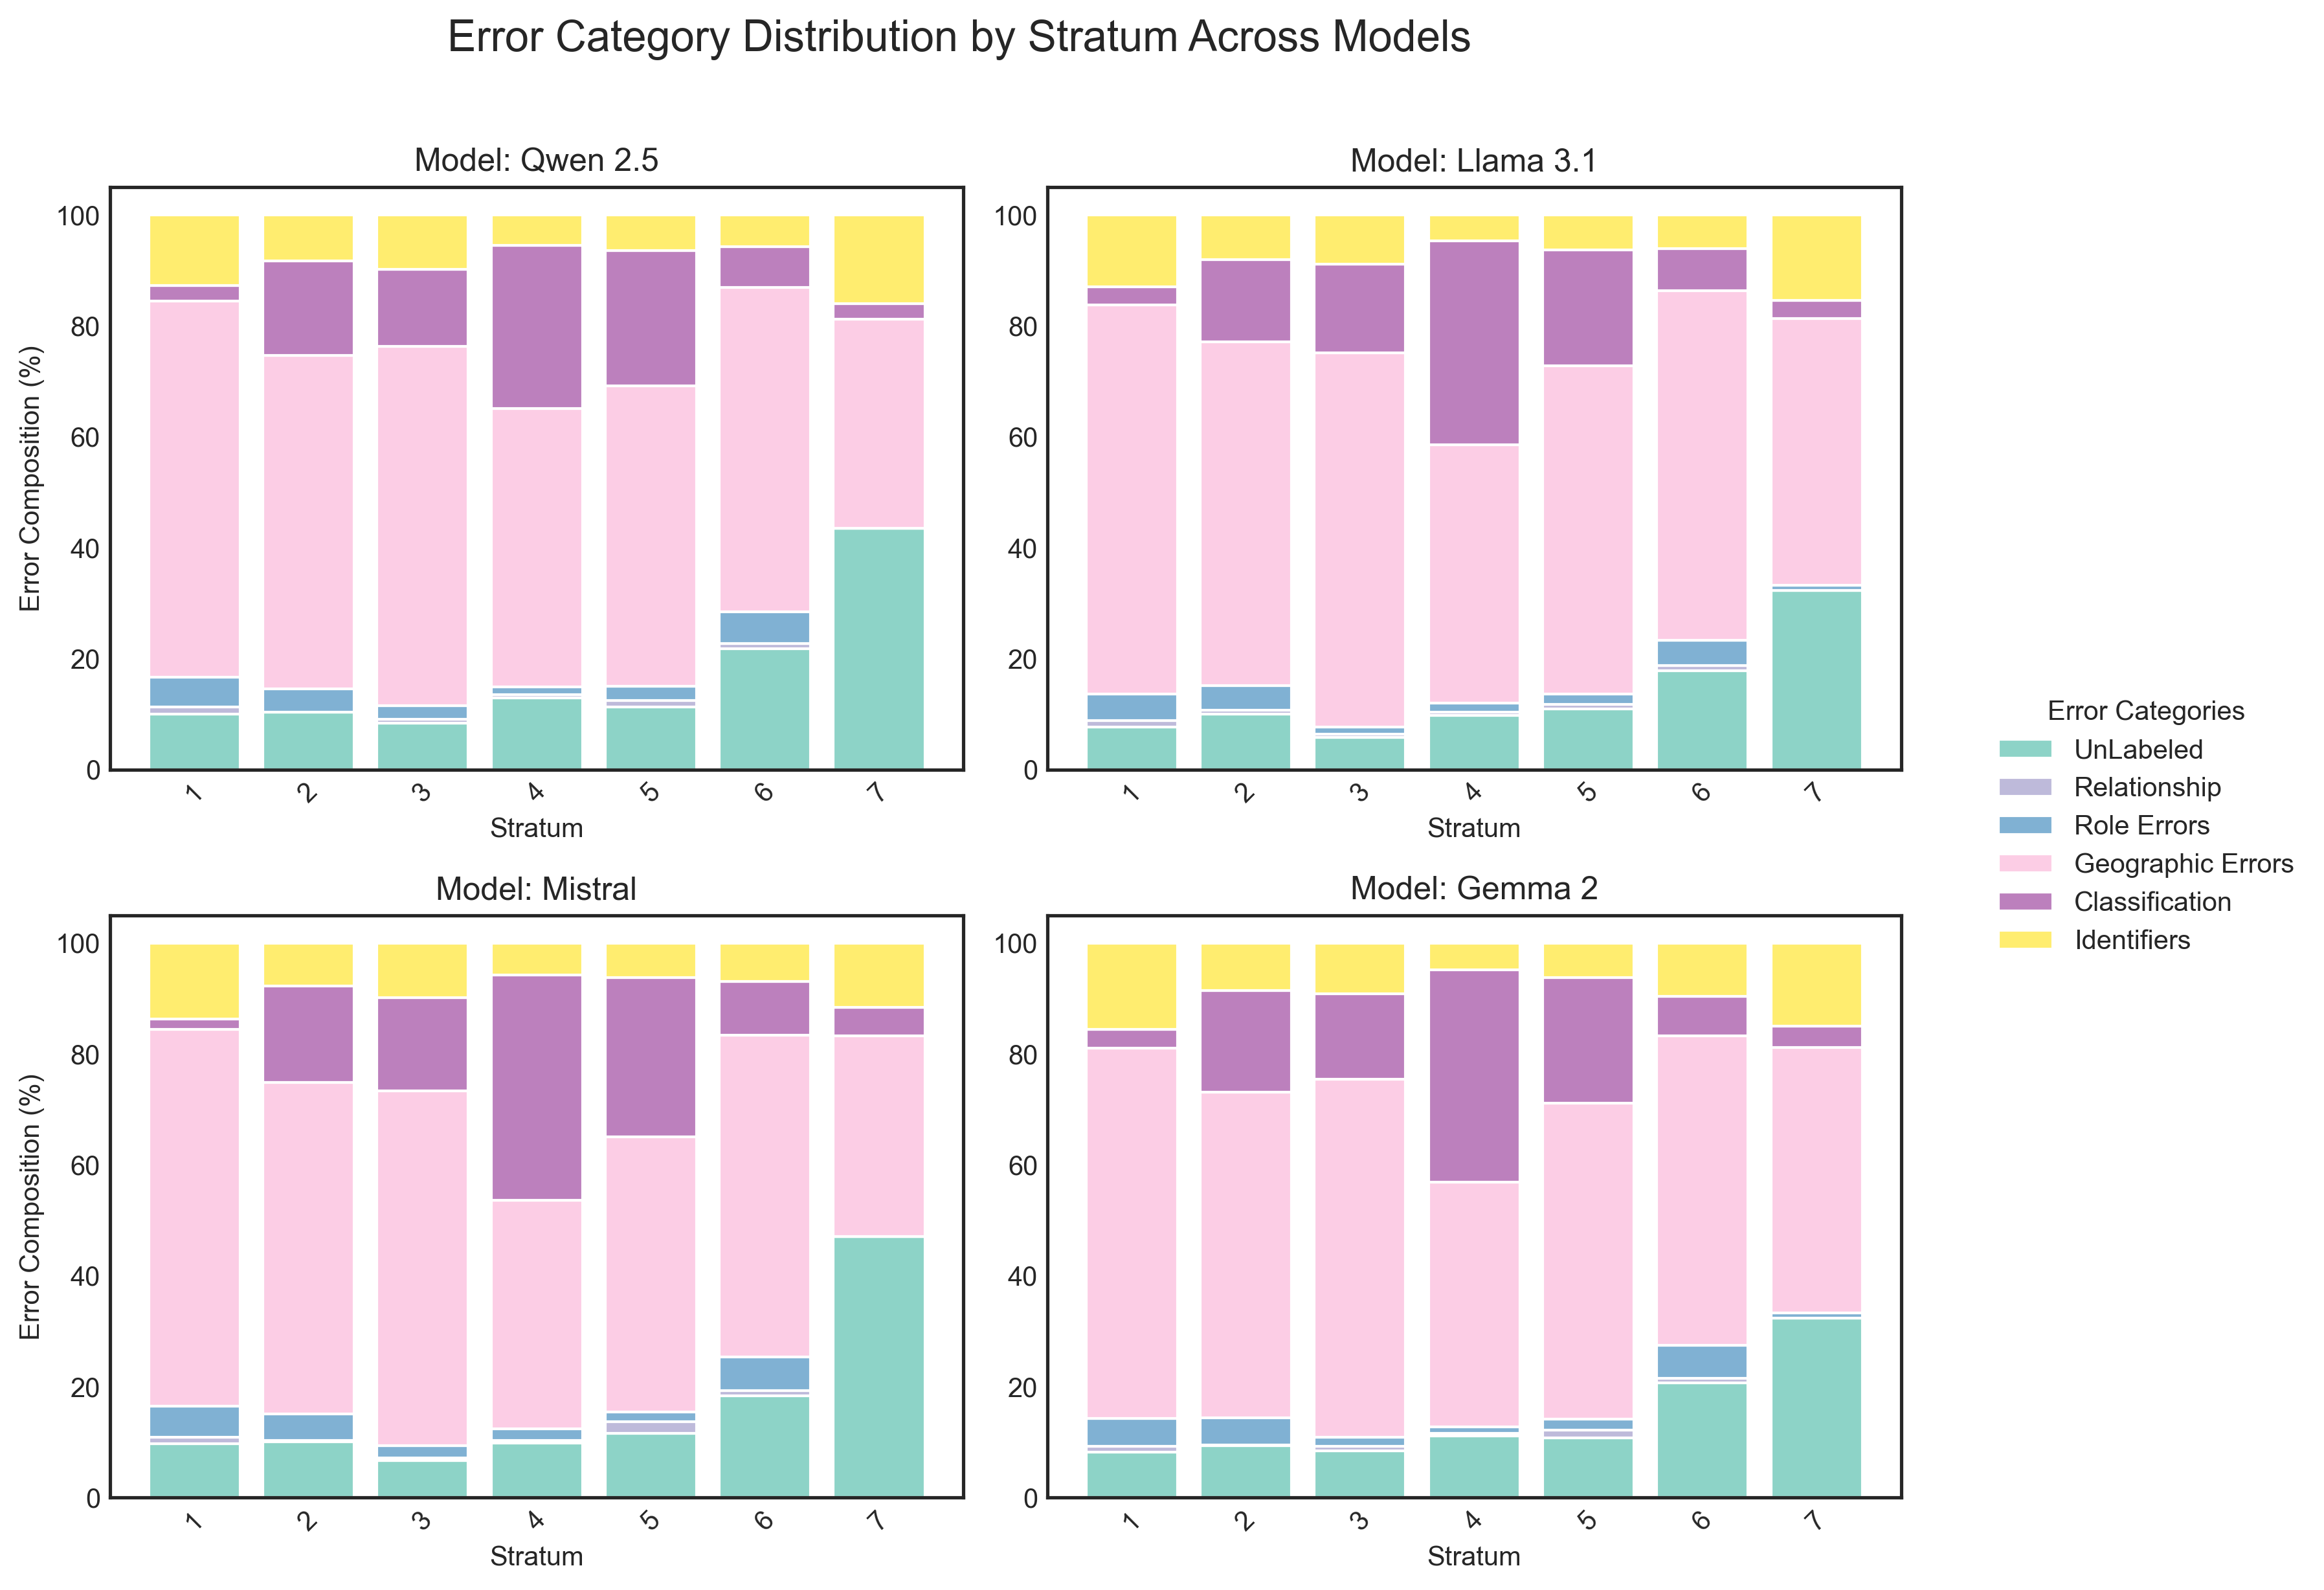
\includegraphics[width=\textwidth]{res/category_distribution_analysis}
    \end{minipage}
    \caption{distribution of error categories across different language models and frequency strata}
    \label{fig:category_distribution_analysis}
\end{figure}

Analysis of error categories in Figure~\ref{fig:category_distribution_analysis} reported separate patterns across strata, with certain error types becoming more prevalent in specific knowledge domains.
The proportion of unLabeled errors increased notably in the most common knowledge strata (6-7), while geographic errors showed higher prevalence in less common knowledge strata (1-3).
Classification errors maintained relatively consistent proportions across all strata, suggesting that this type of error is less influenced by knowledge commonality.

These findings suggest that while newer models like \textit{Qwen2.5} achieve lower overall error rates, they may be more sensitive to knowledge popularity, performing notably better with common knowledge.
In contrast, models like \textit{Gemma2} offer more consistent performance across knowledge types, potentially making them more reliable for applications requiring uniform handling of both common and rare knowledge.

\begin{figure}[ht!]
    \centering
    \begin{minipage}[b]{\textwidth}
        \centering
        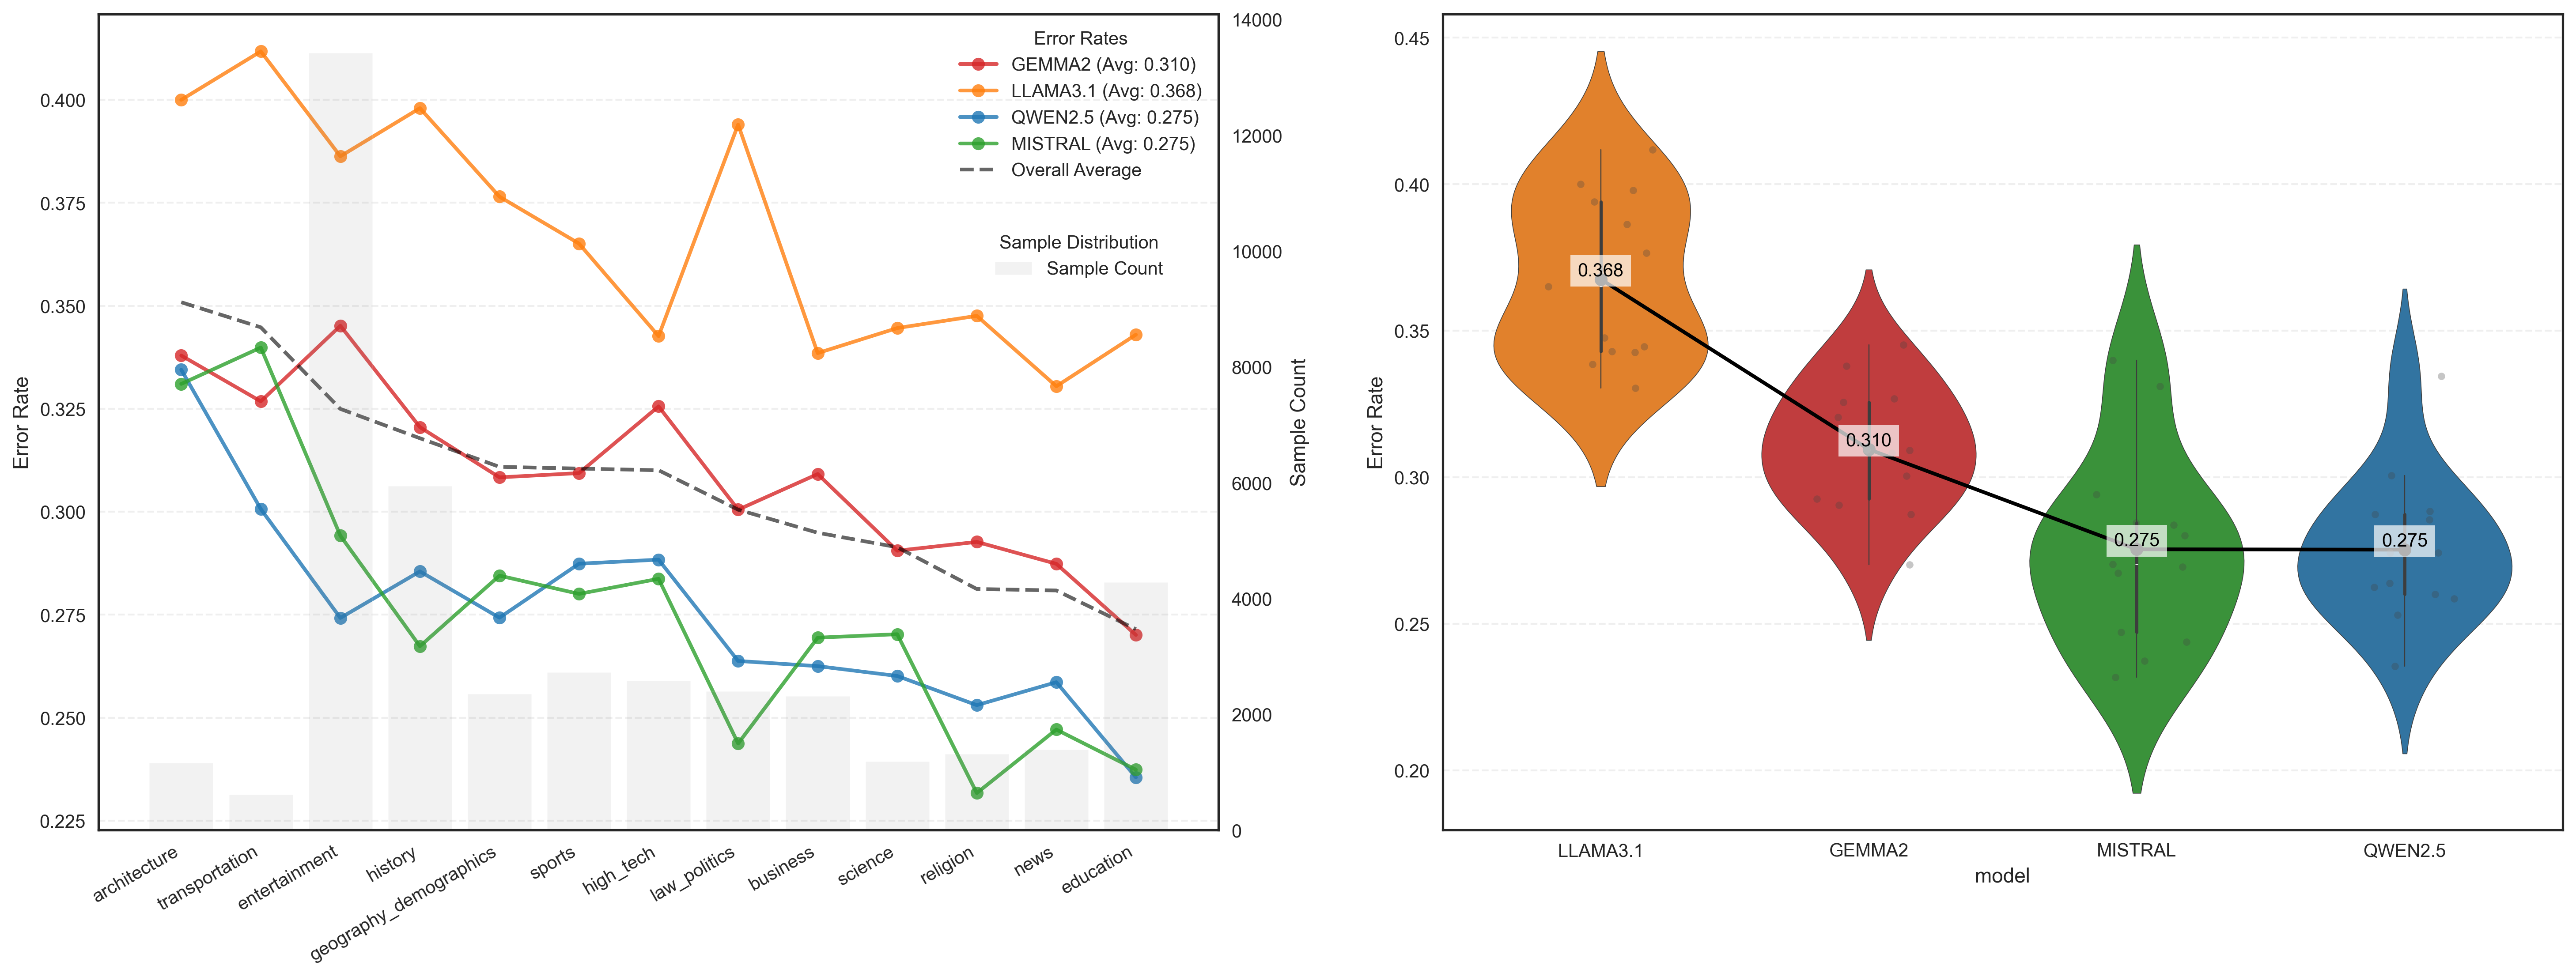
\includegraphics[width=\textwidth]{res/combined-model-analysis}
    \end{minipage}
    \caption{Comparative analysis of language model error rates across knowledge domains. (Left) domain-specific error ratesacross 13 knowledge categories, with overlaid sample distribution bars. (Right) distribution of error rates for each model}
    \label{fig:topic_distribution_analysis}
\end{figure}

By employing BERTopic from the work of Marchesin et al.~\cite{Marchesin_Silvello_Alonso_2024} to generate interpretable clusters, we obtained 64 distinct clusters, which were manually scrutinized and aggregated to form a set of 13 broad topics.
These topics encompass “Architecture", "Business", "Education", "Entertainment", "Geography", "High Tech", "History", "Law and Politics", "News", "Religion", "Science", "Sports", and  "Transportation".
Some facts were not assigned to any topic or were assigned to multiple topics.

As showed in Figure~\ref{fig:topic_distribution_analysis} "Education" and "News" domains consistently show lower error rates across all models.
"Architecture" and "Transportation" categories present higher error rates, particularly for \textit{Llama3.1}.
High variance is observed in the "Business" and "Law and Politics" domains, suggesting these may be more challenging areas for current models.
Also we figured out that \textit{Qwen2.5} and \textit{Mistral} have compact distributions, indicating consistent performance, but \textit{Llama3.1} exhibits the broadest distribution, suggesting more variable performance across domains

Correlation analysis reveals varying relationships between sample count and error rates.
\textit{Gemma2} shows a strong positive correlation (0.410), suggesting lower reliability in less-sampled domains.
\textit{Llama3.1} exhibits a weak positive correlation (0.204).
\textit{Mistral} shows negligible correlation (0.006), indicating consistent performance regardless of sample size.
\textit{Qwen2.5} demonstrates a slight negative correlation (-0.101), hinting at better performance in less-sampled domains.